% ============================================================================
%  Informe - Clasificador normativo de residuos (Resolucion 2184 de 2019)
%  Plantilla: IEEE Signal Processing Society (ieeeconf.cls v1.1)
%  Compilar: pdflatex -> bibtex -> pdflatex -> pdflatex
% ============================================================================
\documentclass[10pt]{ieeeconf}

\usepackage[utf8]{inputenc}
\usepackage[T1]{fontenc}
\usepackage[spanish,es-noshorthands]{babel}
\usepackage{booktabs}
\usepackage{array}
\usepackage{amsmath,amssymb}
\usepackage{graphicx}
\usepackage{xcolor}
\usepackage{tikz}
\usetikzlibrary{positioning,arrows.meta}
\usepackage{microtype}
\usepackage{url}

\graphicspath{{figs/}}

\renewcommand{\abstractname}{Resumen}
\renewcommand{\IEEEkeywordsname}{Palabras clave}
\addto\captionsspanish{\renewcommand{\tablename}{Tabla}}
\renewenvironment{acknowledgments}{\section*{Agradecimientos}}{}

% ----------------------------------------------------------------------------
\title{Del material a la bolsa: clasificaci\'on normativa de residuos s\'olidos
con aprendizaje profundo y abstenci\'on calibrada}

\addauthor{Ariel David Herrera Ahumada}{1}
\addauthor{Jos\'e Arqu\'imedes Soto Monta\~na}{1}
\addaffiliation{1}{Maestr\'ia en Inteligencia Artificial, Universidad de La Salle,
Bogot\'a, Colombia}

\begin{document}
\maketitle

\begin{abstract}
La separaci\'on en la fuente es obligatoria en Colombia desde la Resoluci\'on 2184
de 2019, que organiza los residuos en tres bolsas: blanca (aprovechables), verde
(org\'anicos) y negra (no aprovechables). Sin embargo, la decisi\'on ciudadana
sigue siendo visual y ambigua: una bolsa de pl\'astico sucio, un empaque
metalizado o un textil pueden terminar en la bolsa equivocada y contaminar el
flujo. Este trabajo presenta un clasificador que no responde con el material sino
con la bolsa normativa, y que se abstiene cuando la evidencia no alcanza. Se
comparan dos modelos: A, entrenado sin c\'odigo en Teachable Machine con 180
im\'agenes por clase, y B, MobileNetV3-Small ajustado sobre las 2.951 im\'agenes
de entrenamiento de RealWaste. La proyecci\'on de nueve materiales a tres bolsas
es una tabla normativa, no una clase aprendida. Sobre las 633 im\'agenes
reservadas de \texttt{test/}, el Modelo B alcanza 83,6\,\% de exactitud de
material, 94,9\,\% de bolsa y 0,841 de F1 macro; el Modelo A, 78,2\,\%, 91,9\,\% y
0,777. El umbral $\tau=0{,}63$, calibrado solo en validaci\'on para sostener
90\,\% de exactitud de material, deja al Modelo B decidiendo en el 80,9\,\% de los
casos, con 91,8\,\% de material y 98,2\,\% de bolsa correctos. El sistema completo
se despliega como una imagen Docker con frontend Rust/WASM y API FastAPI/ONNX
Runtime detr\'as de Traefik, con TLS y CI/CD. Una prueba de cambio de dominio con
TrashNet muestra que la exactitud de material cae al 42,4\,\%, lo que delimita el
alcance real del prototipo.
\end{abstract}

\begin{IEEEkeywords}
Clasificaci\'on de residuos, aprendizaje por transferencia, MobileNetV3,
abstenci\'on, Resoluci\'on 2184 de 2019, ONNX Runtime, Rust/WASM.
\end{IEEEkeywords}

% ============================================================================
\section{Introducci\'on}
\label{sec:intro}

Colombia produce residuos s\'olidos urbanos a un ritmo que supera la capacidad de
muchos rellenos sanitarios, y la separaci\'on en la fuente es la primera barrera
para que el material aprovechable no se entierre junto con la basura. La
Resoluci\'on 2184 de 2019 del Ministerio de Ambiente y Desarrollo Sostenible
modific\'o la Resoluci\'on 668 de 2016 y adopt\'o un c\'odigo de colores de
aplicaci\'on nacional: bolsa blanca para residuos aprovechables (pl\'astico,
vidrio, metal, papel y cart\'on limpios), bolsa verde para org\'anicos
aprovechables (restos de comida y poda) y bolsa negra para no aprovechables
(mezclas, contaminados y de un solo uso sucio) \cite{res2184}.

La norma es clara; la decisi\'on frente a un objeto concreto no lo es. Un vaso de
papel con residuos de caf\'e, una bolsa de pl\'astico que contuvo comida o un
empaque multicapa plantean dudas razonables, y el error tiene un costo alto: un
solo residuo contaminado puede invalidar el contenido de una bolsa entera. En
t\'erminos de visi\'on por computador, el problema no es solo clasificar el
material, sino decidir si la evidencia alcanza para decidir. Un clasificador que
siempre responde, aunque su confianza sea baja, traslada al ciudadano un error
que el sistema podr\'ia haber declarado.

Este trabajo construye y eval\'ua un prototipo completo que aborda las dos
decisiones por separado. Primero predice el material con una red convolucional;
despu\'es proyecta las probabilidades a las tres bolsas mediante una tabla
normativa; finalmente se abstiene si la probabilidad m\'axima no supera un umbral
calibrado en validaci\'on. La aplicaci\'on se sirve en el navegador, acepta una
foto o un lote, explica el veredicto y publica la exactitud real del modelo que
est\'a decidiendo.

\subsection{Objetivos}

El objetivo general es dise\~nar, entrenar y desplegar un clasificador de residuos
que traduzca la salida de un modelo de im\'agenes a la decisi\'on normativa de la
Resoluci\'on 2184 y que se abstenga cuando no pueda sostenerla. Los objetivos
espec\'ificos son: (i) preparar una partici\'on reproducible de RealWaste sin
fugas entre entrenamiento y evaluaci\'on; (ii) comparar un modelo entrenado sin
c\'odigo en Teachable Machine con un modelo de aprendizaje por transferencia;
(iii) calibrar el umbral de abstenci\'on sobre validaci\'on y evaluarlo una sola
vez sobre prueba; (iv) medir el cambio de dominio con un conjunto externo; y (v)
desplegar el sistema con TLS, contenedor y pipeline de integraci\'on continua.

\subsection{Contribuciones}

\begin{itemize}
\item Un clasificador que separa la predicci\'on del material de la regla
normativa, de modo que un cambio en la norma no obligue a reentrenar el modelo.
\item Una comparaci\'on controlada entre un modelo sin c\'odigo y un modelo
ajustado, con la misma partici\'on, la misma normalizaci\'on y el mismo umbral.
\item Un umbral de abstenci\'on calibrado sobre exactitud de material, con la
curva cobertura--exactitud publicada y visible en la aplicaci\'on.
\item Un sistema reproducible de punta a punta: scripts de datos, entrenamiento,
evaluaci\'on, conversi\'on a ONNX, API, interfaz y despliegue en un VPS real.
\end{itemize}

El resto del documento se organiza as\'i: la Secci\'on~\ref{sec:marco} presenta
el marco normativo y t\'ecnico; la Secci\'on~\ref{sec:datos} describe los datos y
la partici\'on; la Secci\'on~\ref{sec:metodo} detalla los modelos y la
calibraci\'on; la Secci\'on~\ref{sec:sistema} describe la arquitectura y el
despliegue; la Secci\'on~\ref{sec:resultados} reporta los resultados; la
Secci\'on~\ref{sec:discusion} los discute y la Secci\'on~\ref{sec:conclusiones}
cierra con las conclusiones.

% ============================================================================
\section{Marco de referencia}
\label{sec:marco}

\subsection{La norma y el costo del error}

La Resoluci\'on 2184 de 2019 no solo fija colores: define qu\'e se considera
aprovechable y qu\'e no, y responsabiliza al generador de la separaci\'on en la
fuente. La Tabla~\ref{tab:bolsas} resume la proyecci\'on que usa este trabajo. Dos
aspectos son relevantes para el dise\~no. Primero, la mayor\'ia de los materiales
comparte la bolsa blanca, de modo que acertar la bolsa es m\'as f\'acil que
acertar el material; una m\'etrica de bolsa puede ocultar errores de
clasificaci\'on que s\'i importan al usuario. Segundo, la bolsa negra es la m\'as
heterog\'enea: mezclas, textiles y residuos contaminados no comparten una
apariencia visual, y por eso es la clase con mayor riesgo.

\subsection{Redes convolucionales y aprendizaje por transferencia}

Las redes convolucionales aprenden jerarqu\'ias de filtros a partir de datos
etiquetados. Cuando el corpus es peque\~no, el aprendizaje por transferencia parte
de un modelo preentrenado en ImageNet y ajusta una parte de sus pesos al dominio
objetivo; as\'i se aprovechan bordes, texturas y formas que no dependen de la
tarea. MobileNetV3-Small es una arquitectura dise\~nada para dispositivos con
recursos limitados: combina bloques con conexiones residuales, m\'odulos de
atenci\'on por canal (squeeze-and-excitation) y la no linealidad \textit{h-swish},
y fue encontrada mediante b\'usqueda de arquitecturas \cite{howard2019mobilenetv3}.
Su tama\~no reducido la hace adecuada para servir inferencia en CPU.

Teachable Machine, en cambio, es una herramienta sin c\'odigo que entrena un
modelo de imagen a partir de ejemplos cargados en el navegador
\cite{teachablemachine}. Se usa aqu\'i como l\'inea base: representa lo que un
equipo sin experiencia en entrenamiento puede obtener con el mismo corpus y
constituye una comparaci\'on honesta frente al ajuste fino.

\subsection{Abstenci\'on y calibraci\'on}

La opci\'on de rechazo es un problema cl\'asico de reconocimiento de patrones: el
sistema puede no decidir cuando la evidencia es insuficiente, a cambio de perder
cobertura \cite{chow1970}. En redes modernas, la probabilidad m\'axima de una
softmax no es una medida fiable de correcci\'on; los modelos tienden a ser
sobreconfiados y la calibraci\'on cambia con la profundidad y el r\'egimen de
entrenamiento \cite{guo2017calibration}. Por eso el umbral no se elige a ojo: se
calibra sobre un conjunto de validaci\'on y se congela antes de tocar prueba.

La curva cobertura--exactitud resume el compromiso. Para un umbral $\tau$, la
cobertura $C(\tau)$ es la fracci\'on de im\'agenes aceptadas y la exactitud
condicional $A(\tau)$ es el acierto entre las aceptadas. Al aumentar $\tau$ baja
la cobertura y sube la exactitud; el punto de operaci\'on es una decisi\'on de
riesgo, no una propiedad del modelo.

\subsection{Trabajos relacionados}

TrashNet fue uno de los primeros conjuntos p\'ublicos para clasificar residuos
reciclables y sigue us\'andose como referencia, aunque sus imágenes se tomaron
sobre fondo blanco y en condiciones controladas \cite{thung2016trashnet}.
RealWaste se recolect\'o en un relleno sanitario real, con iluminaci\'on, suciedad
y fondos variables, y por eso es un banco de prueba m\'as cercano al uso
ciudadano \cite{single2023realwaste}. La mayor\'ia de los trabajos reporta
exactitud de material sobre una partici\'on del propio conjunto; son menos los que
reportan la decisi\'on normativa, la abstenci\'on y el comportamiento en un
dominio distinto. Este trabajo reporta las tres cosas y separa expl\'icitamente la
capa aprendida de la capa normativa.

% ============================================================================
\section{Datos y preparaci\'on}
\label{sec:datos}

\subsection{RealWaste}

RealWaste contiene 4.752 im\'agenes de 524$\times$524 p\'ixeles en nueve clases de
material, capturadas en el punto de recepci\'on de un relleno sanitario
\cite{realwasteuci}. La Tabla~\ref{tab:realwaste} muestra el conteo original y el
conteo despu\'es de eliminar duplicados. El desbalance es notable: Pl\'astico
concentra 921 im\'agenes originales y Textil 318, una proporci\'on de casi tres a
uno. Esa asimetr\'ia se refleja en la partici\'on y obliga a usar pesos por clase
en la p\'erdida del Modelo B.

\begin{table}[t]
\centering
\caption{RealWaste: im\'agenes por clase antes y despu\'es de la deduplicaci\'on,
y reparto final entre entrenamiento, validaci\'on y prueba. Validaci\'on y prueba
comparten el mismo conteo por clase.}
\label{tab:realwaste}
\footnotesize
\setlength{\tabcolsep}{3.5pt}
\begin{tabular}{@{}lrrrr@{}}
\toprule
Clase & Original & \'Unicas & train & val/test \\
\midrule
Cart\'on            & 461 & 433 & 303 & 65 \\
Org\'anicos         & 411 & 394 & 276 & 59 \\
Vidrio              & 420 & 345 & 241 & 52 \\
Metal               & 790 & 616 & 432 & 92 \\
No aprovechable     & 495 & 435 & 305 & 65 \\
Papel               & 500 & 457 & 319 & 69 \\
Pl\'astico          & 921 & 832 & 582 & 125 \\
Textil              & 318 & 281 & 197 & 42 \\
Vegetaci\'on        & 436 & 424 & 296 & 64 \\
\midrule
Total               & 4.752 & 4.217 & 2.951 & 633 \\
\bottomrule
\end{tabular}
\end{table}

\subsection{TrashNet}

TrashNet re\'une 2.527 im\'agenes en seis clases: vidrio (501), papel (594),
cart\'on (403), pl\'astico (482), metal (410) y basura mezclada (137). Las fotos
se tomaron sobre un fondo blanco con iluminaci\'on controlada, lo que introduce un
cambio de dominio fuerte frente a RealWaste. Se usa \'unicamente como prueba
externa: no participa en entrenamiento ni en calibraci\'on. Para la exactitud de
material se consideran las cinco clases compartidas; \textit{trash} se excluye
porque agrupa mezclas sin un material \'unico. Para la decisi\'on de bolsa s\'i
entra, con destino en la bolsa negra.

\subsection{Deduplicaci\'on y partici\'on}

Los conjuntos de im\'agenes de residuos suelen contener la misma foto repetida,
variantes redimensionadas o r\'afagas de un mismo objeto. Si esas variantes caen
en lados distintos de la partici\'on, la exactitud de prueba se infla. Para
evitarlo se calcul\'o una huella dHash de 64 bits sobre cada imagen y se
eliminaron las que ten\'ian distancia de Hamming menor o igual a 6 respecto de
una ya conservada. El filtro retir\'o 535 im\'agenes (11,3\,\%), y la partici\'on
se hizo despu\'es, de forma estratificada por clase y con semilla fija.

El resultado es 2.951 im\'agenes de entrenamiento, 633 de validaci\'on y 633 de
prueba (70/15/15). El manifiesto \texttt{datos/manifiesto.csv} es la fuente de
verdad: cada fila declara la ruta, la clase, el material, la bolsa y la parte, y
ning\'un script vuelve a repartir. La partici\'on es reproducible con la misma
semilla y est\'a cubierta por pruebas automatizadas que verifican que ninguna
clase quede vac\'ia en validaci\'on o prueba.

\subsection{Proyecci\'on normativa}

La Tabla~\ref{tab:proyeccion} define la capa que traduce material a bolsa. Es una
tabla declarada en el dominio, no una salida del modelo. Esta separaci\'on tiene
dos consecuencias: el modelo puede compararse con la literatura de materiales, y
un cambio normativo se resuelve editando la tabla, sin reentrenar.

\begin{table}[t]
\centering
\caption{Proyecci\'on de las nueve clases de RealWaste a las tres bolsas de la
Resoluci\'on 2184 de 2019.}
\label{tab:proyeccion}
\footnotesize
\begin{tabular}{@{}lll@{}}
\toprule
Clase del modelo & Material & Bolsa \\
\midrule
Cardboard & Cart\'on & Blanca \\
Food Organics & Org\'anicos & Verde \\
Glass & Vidrio & Blanca \\
Metal & Metal & Blanca \\
Miscellaneous Trash & No aprovechable & Negra \\
Paper & Papel & Blanca \\
Plastic & Pl\'astico & Blanca \\
Textile Trash & Textil & Negra \\
Vegetation & Vegetaci\'on & Verde \\
\bottomrule
\end{tabular}
\end{table}

\subsection{An\'alisis exploratorio}

La Fig.~\ref{fig:eda_clases} muestra el conteo por clase, con el color de la
bolsa normativa de cada material. La Fig.~\ref{fig:eda_bolsas} revela el sesgo
normativo del corpus: el 63,6\,\% de las im\'agenes va a la bolsa blanca, el
19,4\,\% a la verde y el 17,0\,\% a la negra, y muestra que la estratificaci\'on
70/15/15 conserva esa proporci\'on en las tres particiones. La
Fig.~\ref{fig:mosaico} contrasta muestras de RealWaste y de TrashNet: el primero
tiene fondos y escalas variables; el segundo, un fondo blanco uniforme. Esa
diferencia anticipa el resultado de la prueba externa.

\begin{figure}[!tb]
\centering
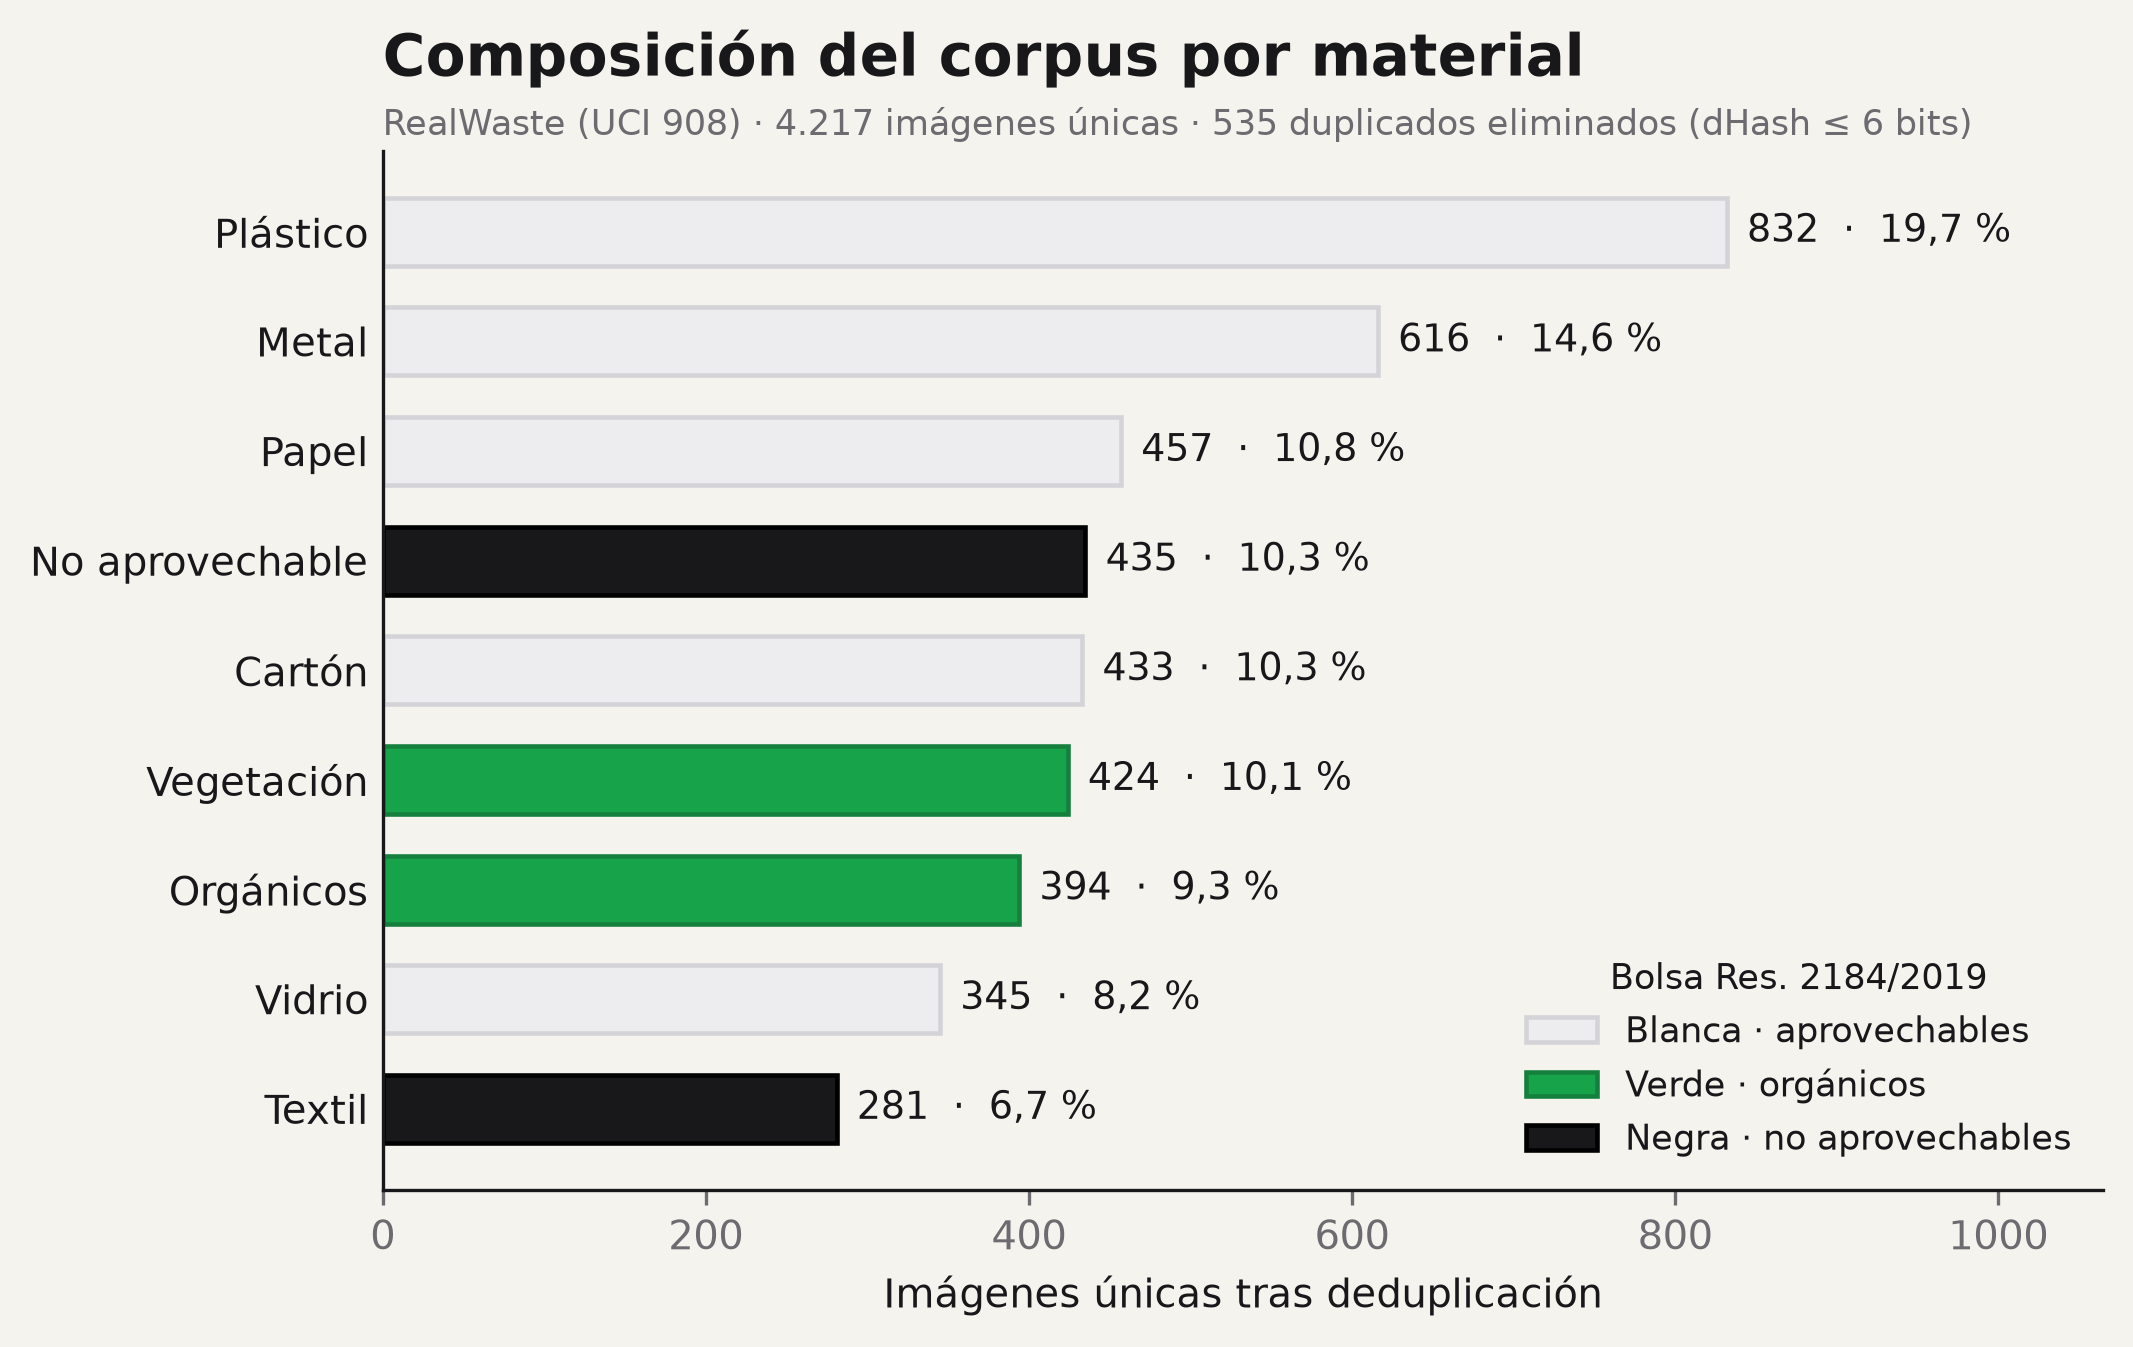
\includegraphics[width=\columnwidth]{eda_clases.png}
\caption{Composici\'on del corpus por material; el color indica la bolsa
normativa de cada clase.}
\label{fig:eda_clases}
\end{figure}

\begin{figure}[!tb]
\centering
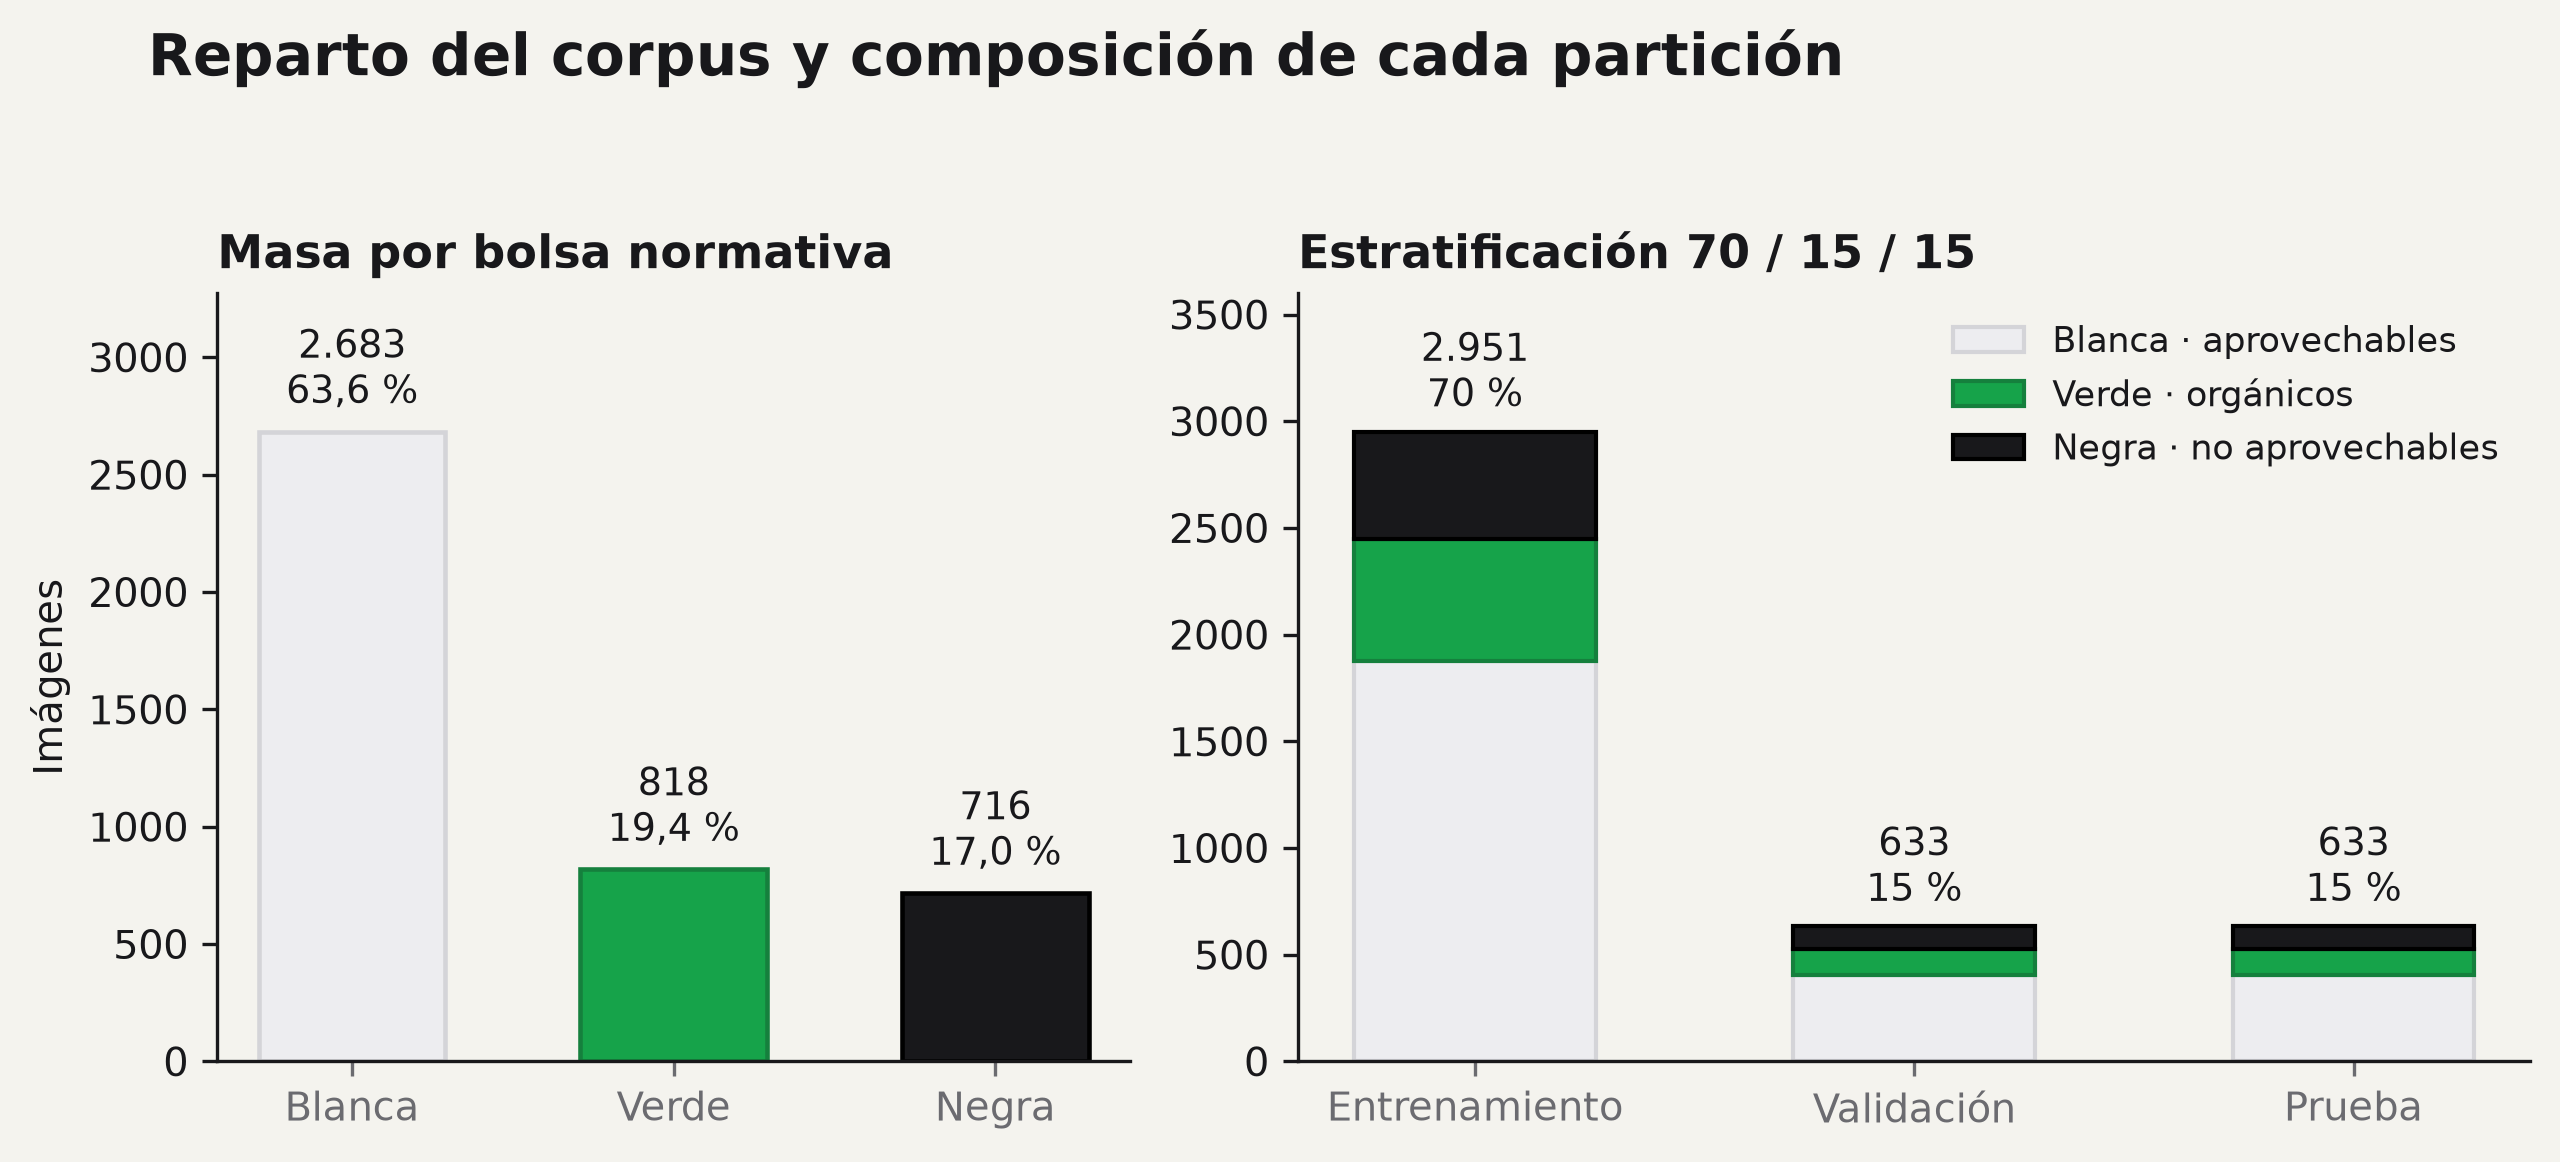
\includegraphics[width=\columnwidth]{eda_bolsas.png}
\caption{Masa de cada bolsa normativa y reparto estratificado del corpus entre
entrenamiento, validaci\'on y prueba. La bolsa blanca concentra el 63,6\,\% del
corpus.}
\label{fig:eda_bolsas}
\end{figure}

\begin{figure}[!tb]
\centering
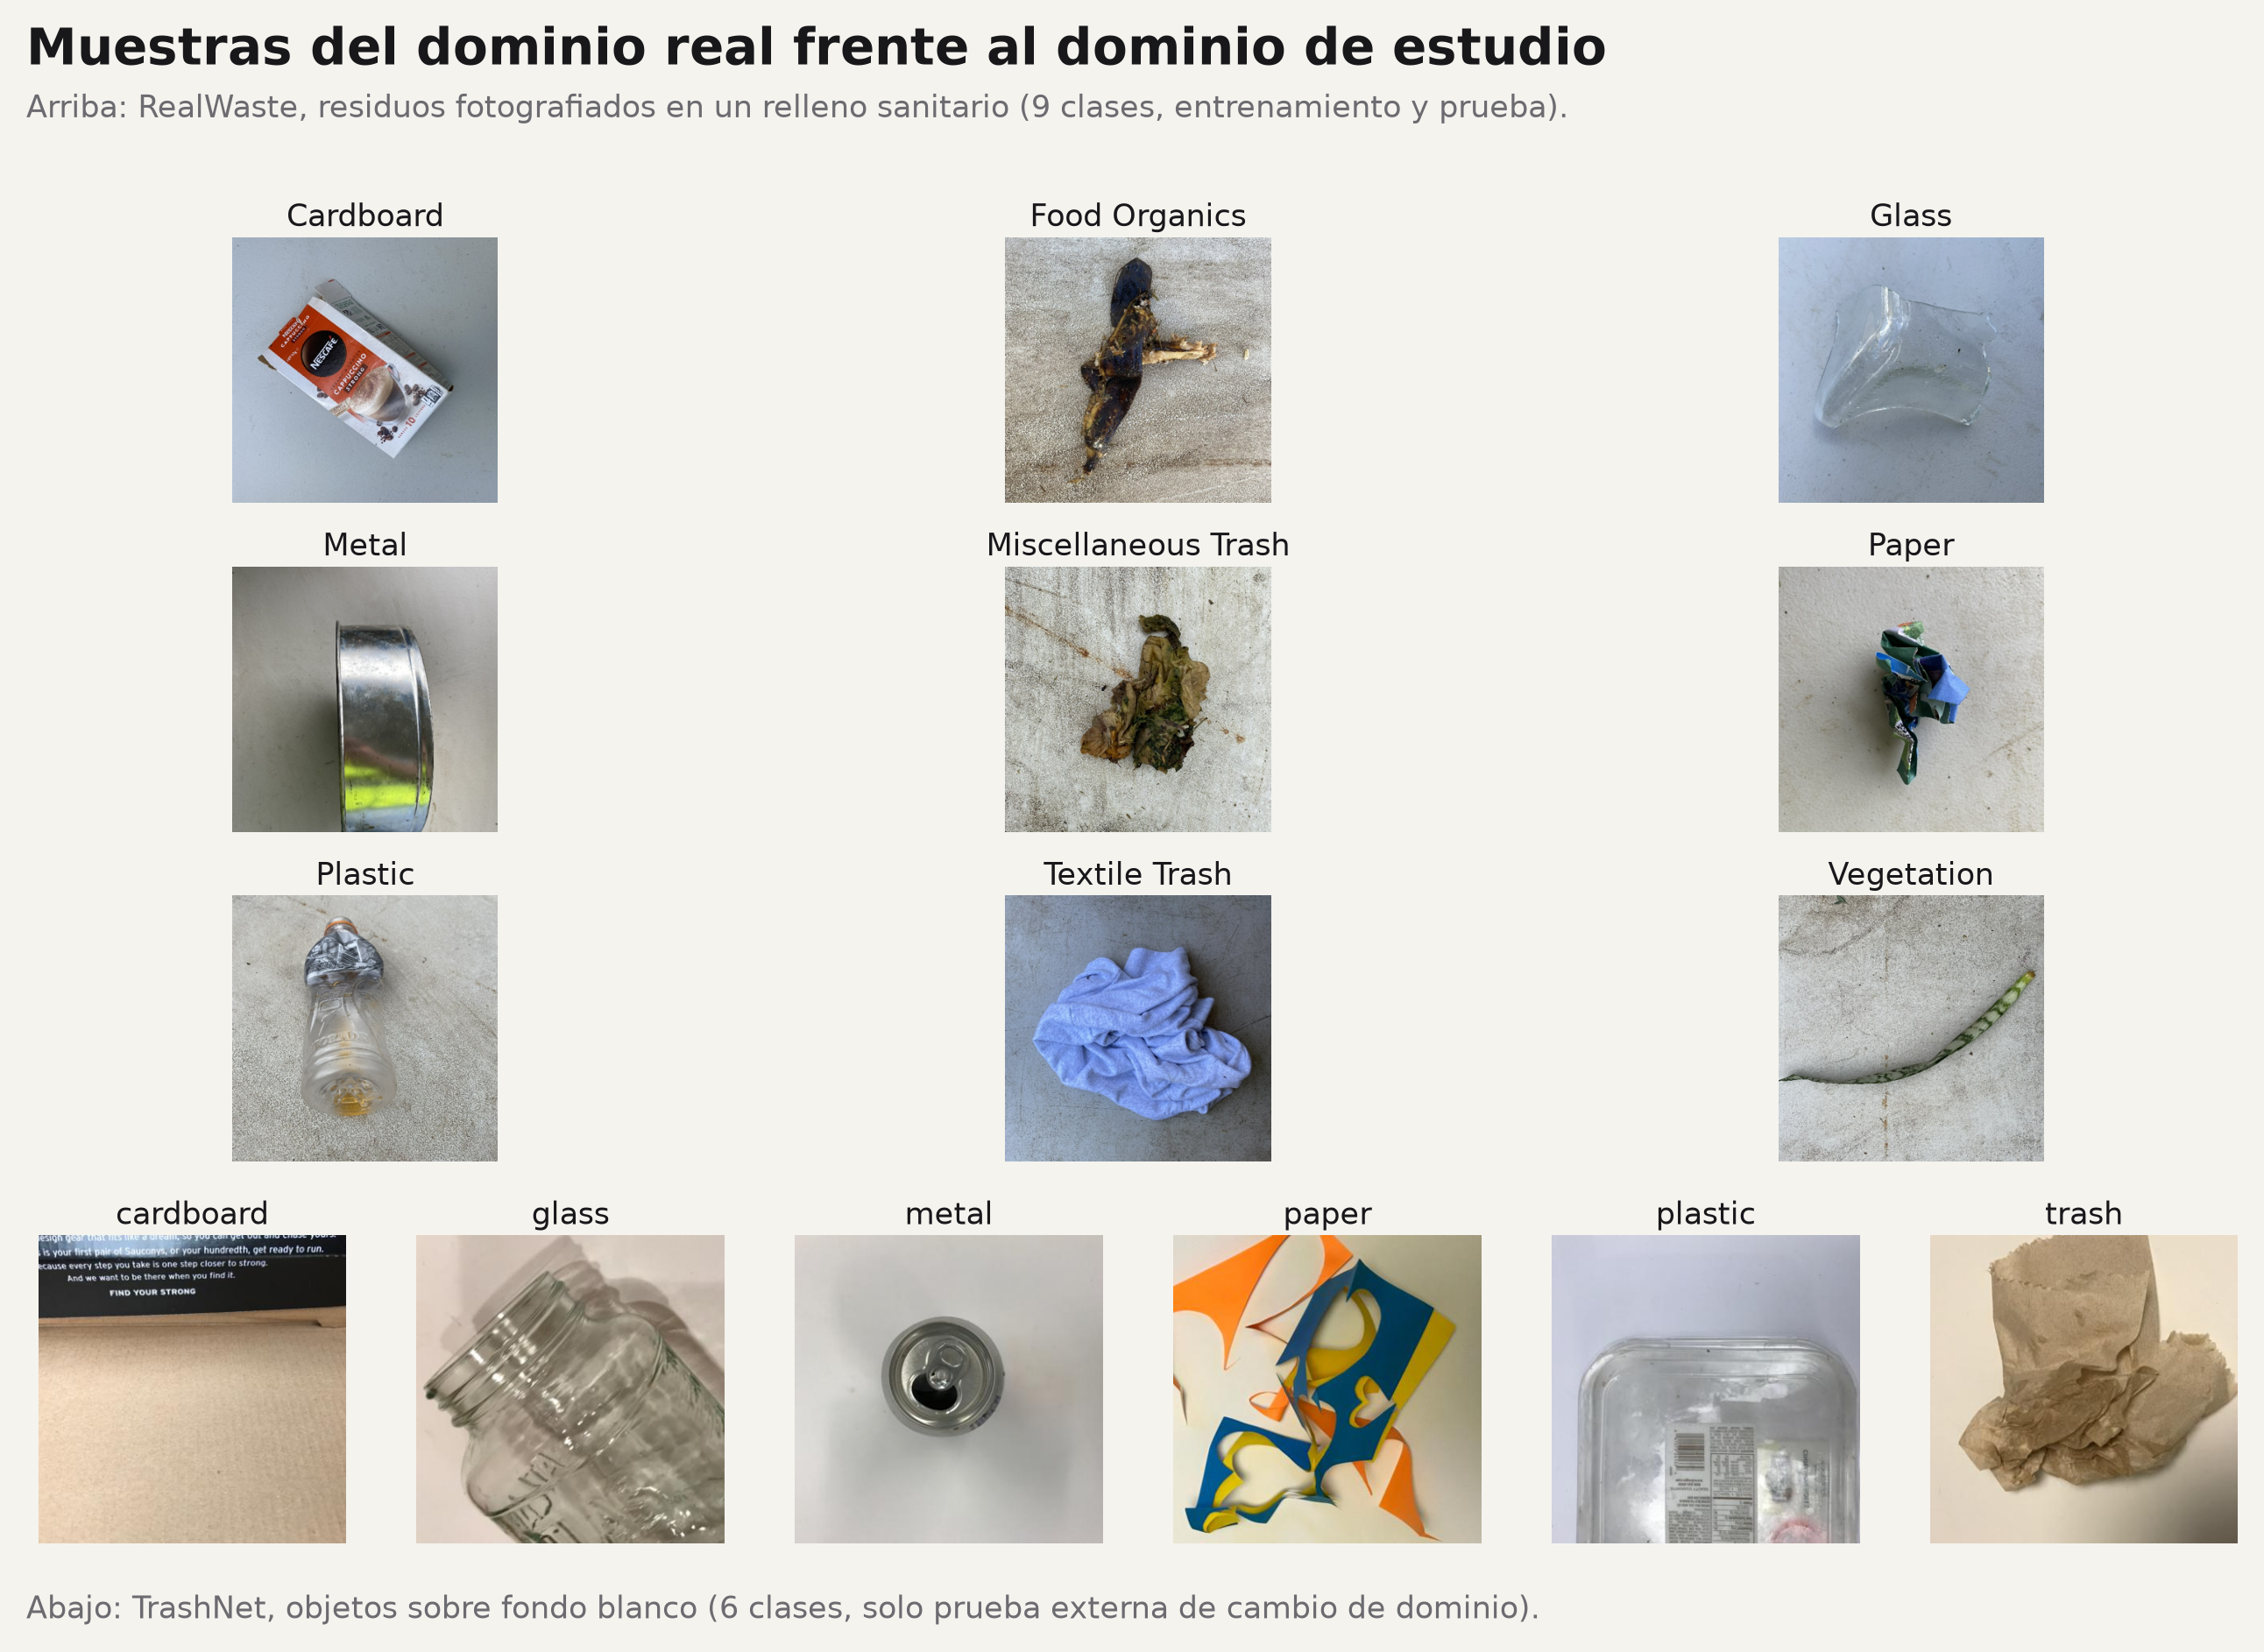
\includegraphics[width=\columnwidth]{eda_mosaico.png}
\caption{Muestras de RealWaste (arriba) y de TrashNet (abajo). El cambio de
fondo, iluminaci\'on y escala es evidente.}
\label{fig:mosaico}
\end{figure}

\subsection{Licencia y consideraciones \'eticas}

RealWaste se distribuye con licencia CC BY 4.0 y TrashNet con fines acad\'emicos.
Las im\'agenes no contienen personas ni datos personales. La aplicaci\'on no
almacena las fotos que recibe: se procesan en memoria y se descartan al responder
la petici\'on. El prototipo es una ayuda a la decisi\'on y no sustituye la norma
municipal ni el criterio de la autoridad ambiental.

% ============================================================================
\section{Metodolog\'ia}
\label{sec:metodo}

\subsection{Visi\'on general}

La Fig.~\ref{fig:pipeline} resume el flujo. Los datos crudos se deduplican y se
parten una sola vez; el Modelo A se entrena en Teachable Machine con un
subconjunto de 180 im\'agenes por clase y el Modelo B se ajusta sobre todo
\texttt{train/}. El umbral se calibra en \texttt{val/} y se congela; la
evaluaci\'on se ejecuta una sola vez sobre \texttt{test/} y sobre TrashNet. Los
dos modelos se exportan a ONNX y la API elige el B si est\'a presente.

\begin{figure}[!tb]
\centering
\begin{tikzpicture}[
  caja/.style={draw, rounded corners=2pt, align=center, font=\footnotesize,
    text width=0.74\columnwidth, inner sep=4pt},
  flecha/.style={-{Stealth[length=2mm]}, thick}
]
\node[caja] (a) {RealWaste (4.752) + TrashNet (2.527)};
\node[caja, below=4mm of a] (b) {dHash $\le 6$ bits y partici\'on 70/15/15\\
  4.217 im\'agenes, manifiesto CSV};
\node[caja, below=4mm of b] (c) {Modelo A: Teachable Machine\\
  1.620 im\'agenes, 50 \'epocas};
\node[caja, below=4mm of c] (d) {Modelo B: MobileNetV3-Small\\
  2.951 im\'agenes, 12 \'epocas};
\node[caja, below=4mm of d] (e) {Calibraci\'on de $\tau$ en \texttt{val/}\\
  $\tau^\star = 0{,}63$};
\node[caja, below=4mm of e] (f) {Evaluaci\'on \'unica en \texttt{test/}\\
  y prueba externa TrashNet};
\node[caja, below=4mm of f] (g) {Export ONNX $\rightarrow$ FastAPI + WASM\\
  $\rightarrow$ GHCR $\rightarrow$ VPS con Traefik};
\foreach \x/\y in {a/b,b/c,c/d,d/e,e/f,f/g} \draw[flecha] (\x) -- (\y);
\end{tikzpicture}
\caption{Flujo reproducible del proyecto. Cada etapa tiene un script y deja un
archivo verificable.}
\label{fig:pipeline}
\end{figure}

\subsection{Modelo A: Teachable Machine}

Se cargaron 180 im\'agenes por clase, ya redimensionadas a 224$\times$224, en la
interfaz de Teachable Machine. La configuraci\'on fue la predeterminada de la
herramienta para im\'agenes: 50 \'epocas, lote de 16 y tasa de aprendizaje
0,001. El modelo exportado en formato Keras se convirti\'o a ONNX con
\texttt{tf2onnx} y se verific\'o que la diferencia m\'axima entre ambas salidas
fuera menor o igual a $10^{-4}$; si la conversi\'on no reproduce al original, el
script falla y el modelo no llega a la aplicaci\'on.

\subsection{Modelo B: MobileNetV3-Small ajustado}

Se parti\'o de MobileNetV3-Small preentrenada en ImageNet. Se congelaron todos los
pesos y se descongelaron los dos \'ultimos bloques de caracter\'isticas y el
clasificador. El entrenamiento us\'o AdamW con tasa $3\times10^{-4}$, decaimiento
de peso $10^{-4}$ y un planificador coseno durante 12 \'epocas, lote de 32 y
semilla 42. La p\'erdida fue entrop\'ia cruzada con pesos inversos a la frecuencia
de cada clase, para compensar el desbalance de RealWaste. El aumento de datos
incluy\'o recorte aleatorio con escala 0,65--1,0, volteo horizontal, rotaci\'on de
hasta 15$^\circ$ y variaci\'on de brillo, contraste y saturaci\'on de 0,2.

La Tabla~\ref{tab:hiper} contrasta las dos configuraciones. La diferencia de
datos es deliberada: el Modelo A representa el l\'imite de una herramienta sin
c\'odigo con 180 ejemplos por clase; el Modelo B, lo que se obtiene al usar todo
el corpus disponible.

\begin{table}[t]
\centering
\caption{Configuraci\'on de los dos modelos.}
\label{tab:hiper}
\footnotesize
\setlength{\tabcolsep}{3pt}
\begin{tabular}{@{}lcc@{}}
\toprule
 & Modelo A & Modelo B \\
\midrule
Origen & Teachable Machine & ImageNet \\
Arquitectura & Keras (TM) & MobileNetV3-S \\
Im\'agenes de train & 1.620 & 2.951 \\
\'Epocas & 50 & 12 \\
Lote & 16 & 32 \\
Tasa & 0,001 & $3\times10^{-4}$ \\
Optimizador & Adam & AdamW \\
Aumento & el de TM & moderado \\
Pesos por clase & no & s\'i \\
\bottomrule
\end{tabular}
\end{table}

\subsection{Una sola normalizaci\'on}

El Modelo B se entren\'o con media y desviaci\'on 0,5, es decir, la misma
transformaci\'on $x/127{,}5-1$ que usa la API para el Modelo A. La alternativa
--normalizar con la media y desviaci\'on de ImageNet-- habr\'ia obligado a que la
API eligiera el preprocesado seg\'un el archivo cargado, con dos caminos que se
pueden desincronizar. Con una sola normalizaci\'on, el tensor que arma la API
sirve para cualquiera de los dos ONNX y la comparaci\'on A/B mide modelos, no
diferencias de preprocesado.

\subsection{Calibraci\'on del umbral}

Sea $p_i$ la probabilidad del material $i$ y $\beta(i)$ la bolsa a la que
pertenece. La proyecci\'on normativa es
\begin{equation}
P(B_b) = \sum_{i:\,\beta(i)=b} p_i,
\label{eq:bolsa}
\end{equation}
y la decisi\'on con abstenci\'on es
\begin{equation}
\hat{y} =
\begin{cases}
\arg\max_i p_i, & \max_i p_i \ge \tau,\\
\text{abstenci\'on}, & \text{en otro caso}.
\end{cases}
\label{eq:tau}
\end{equation}
El umbral se eligi\'o sobre \texttt{val/} como el menor valor que sostiene al
menos 90\,\% de exactitud de material entre las im\'agenes aceptadas:
\begin{equation}
\tau^\star = \min\left\{\tau : A_{\text{mat}}(\tau) \ge 0{,}90\right\},
\label{eq:tauopt}
\end{equation}
donde $A_{\text{mat}}(\tau)$ se calcula solo con las im\'agenes cuya probabilidad
m\'axima alcanza $\tau$. La calibraci\'on se hizo sobre material y no sobre bolsa
por una raz\'on concreta: como cinco de las nueve clases van a la bolsa blanca,
la exactitud de bolsa es alta incluso cuando el material est\'a mal. Calibrado
sobre bolsa, el barrido elige $\tau=0{,}30$ con 92,5\,\% de acierto, pero acepta
el 99,7\,\% de las im\'agenes y la abstenci\'on queda decorativa. Calibrado sobre
material, el umbral calla cuando el modelo no distingue un cart\'on de un
pl\'astico, aunque ambos vayan a la misma bolsa.

La cobertura se reporta como
\begin{equation}
C(\tau) = \frac{1}{N}\sum_{n=1}^{N}\mathbf{1}\left[\max_i p_{ni} \ge \tau\right].
\label{eq:cobertura}
\end{equation}

\subsection{Conversi\'on a ONNX y el doble softmax}

Los dos modelos se sirven con ONNX Runtime \cite{onnxruntime}. La conversi\'on
introdujo un error sutil que vale la pena documentar: el SavedModel de Teachable
Machine termina en una capa softmax y \texttt{tf2onnx} la conserva, mientras que
el modelo de PyTorch termina en logits. Al aplicar softmax a una salida que ya era
una distribuci\'on, el Modelo A quedaba aplanado: su probabilidad m\'axima casi
nunca pasaba de 0,63 y la bolsa predicha era siempre la blanca. La exactitud de
material no se mov\'ia, porque el argmax es invariante a una transformaci\'on
mon\'otona, pero la abstenci\'on y la proyecci\'on a bolsas s\'i. La API ahora
detecta al cargar si la salida cruda ya es una distribuci\'on (componentes no
negativas que suman uno) y solo aplica softmax cuando recibe logits. Con la
correcci\'on, el Modelo A pas\'o de 63,7\,\% a 91,9\,\% de exactitud de bolsa y su
log-loss baj\'o de 1,60 a 0,98. Una prueba con grafos ONNX m\'inimos cubre los dos
casos para que la regresi\'on no vuelva.

\subsection{M\'etricas}

Se reportan exactitud de material, exactitud top-2, log-loss, precisi\'on, recall
y F1 macro, AUC uno-contra-el-resto y exactitud de bolsa. La F1 macro trata las
nueve clases por igual y no deja que Pl\'astico, la clase mayoritaria, domine el
promedio. La exactitud de bolsa se calcula despu\'es de sumar la masa de
probabilidad de cada material en su bolsa. Para la abstenci\'on se reportan
cobertura y exactitud condicional, tanto de material como de bolsa. Todas las
cifras de prueba provienen de una sola pasada de \texttt{src/s06\_evaluar.py} con
el $\tau$ congelado; el conjunto de prueba no se us\'o para elegir hiperpar\'ametros
ni umbral.

% ============================================================================
\section{Arquitectura del sistema}
\label{sec:sistema}

\subsection{Componentes}

El sistema tiene cuatro capas. La capa de dominio declara los nueve materiales,
las tres bolsas y la funci\'on que decide; no importa FastAPI ni ONNX. La capa de
inferencia carga el ONNX, preprocesa la imagen y devuelve probabilidades. La capa
HTTP expone el contrato y sirve los est\'aticos. La capa de interfaz es una
aplicaci\'on Leptos compilada a WebAssembly que consume el mismo origen. El
contenedor final combina el binario WASM y el runtime de Python en una sola
imagen, de modo que no hay CORS ni un segundo servicio que operar.

\subsection{Dominio}

La funci\'on \texttt{decidir(probs, tau)} devuelve el material ganador, la bolsa
de mayor masa, la confianza, el top-3 y las probabilidades por bolsa. Si la
confianza es menor que $\tau$, el material se devuelve como nulo y la respuesta
marca \texttt{abstenido=true}; la bolsa sugerida sigue siendo la de mayor masa,
pero la interfaz la presenta como una sugerencia a revisar, no como un veredicto.
La comparaci\'on es estricta: un valor exactamente igual a $\tau$ decide, lo que
est\'a cubierto por una prueba de borde.

\subsection{Contrato HTTP}

La Tabla~\ref{tab:api} resume los cuatro puntos de entrada. \texttt{/api/predict}
recibe un archivo y un umbral opcional; \texttt{/api/predict-lote} recibe varios
archivos y agrega conteos por bolsa y por material, adem\'as de los abstenidos.
Los archivos se limitan a 12 MB y se rechazan con 400 si no se pueden decodificar.
La respuesta individual incluye nombre del material, bolsa, r\'otulo, colores,
confianza, top-3, probabilidades por bolsa y latencia. \texttt{/api/catalogo}
publica los materiales, las bolsas, el $\tau$ sugerido y las m\'etricas del modelo
activo; \texttt{/api/health} responde con el nombre del modelo y el n\'umero de
clases.

\begin{table}[t]
\centering
\caption{Contrato HTTP de la API.}
\label{tab:api}
\scriptsize
\setlength{\tabcolsep}{3pt}
\begin{tabular}{@{}>{\raggedright\arraybackslash}p{0.31\columnwidth}>{\raggedright\arraybackslash}p{0.59\columnwidth}@{}}
\toprule
Ruta & Entrada y salida \\
\midrule
\texttt{/api/health} & GET. Modelo activo y n\'umero de clases. \\
\texttt{/api/catalogo} & GET. Materiales, bolsas, $\tau$ y m\'etricas. \\
\texttt{/api/predict} & POST. \texttt{archivo}, \texttt{tau}; una decisi\'on. \\
\texttt{/api/predict-lote} & POST. \texttt{archivos}, \texttt{tau}; conteos y lista. \\
\bottomrule
\end{tabular}
\end{table}

\subsection{Interfaz}

La interfaz se escribi\'o en Rust con Leptos en modo cliente y se compila con
\texttt{trunk} \cite{leptos}. La direcci\'on visual es un cartel de imprenta:
papel c\'alido, bordes negros de dos p\'ixeles, sombra dura y tipograf\'ia Archivo
Black para el veredicto. El bloque del veredicto toma el color de la bolsa y
escribe su nombre, de modo que el color nunca es la \'unica se\~nal. La
Fig.~\ref{fig:ui_veredicto} muestra el estado con una foto y la
Fig.~\ref{fig:ui_abstencion} el estado de abstenci\'on con el umbral en 0,90.

El control de exigencia va de 0,30 a 0,90 en pasos de 0,01 y arranca en el
$\tau$ que publica el cat\'alogo (0,63), con un texto en lenguaje llano que
explica qu\'e significa. El panel muestra la confianza, las tres probabilidades
mayores y la masa por bolsa. El lote acepta varias fotos y resume cu\'antas van a
cada bolsa y cu\'antas quedaron sin decidir (Fig.~\ref{fig:ui_lote}). Al pie se
imprime la exactitud real del modelo activo, le\'ida de \texttt{metrics.json}; si
el archivo falta, la frase no se muestra y la aplicaci\'on nunca inventa una
cifra. La Fig.~\ref{fig:ui_movil} muestra la vista m\'ovil; en el tel\'efono el
selector de archivos abre la c\'amara o la galer\'ia, y por eso el despliegue
exige HTTPS.

\begin{figure*}[t]
\centering
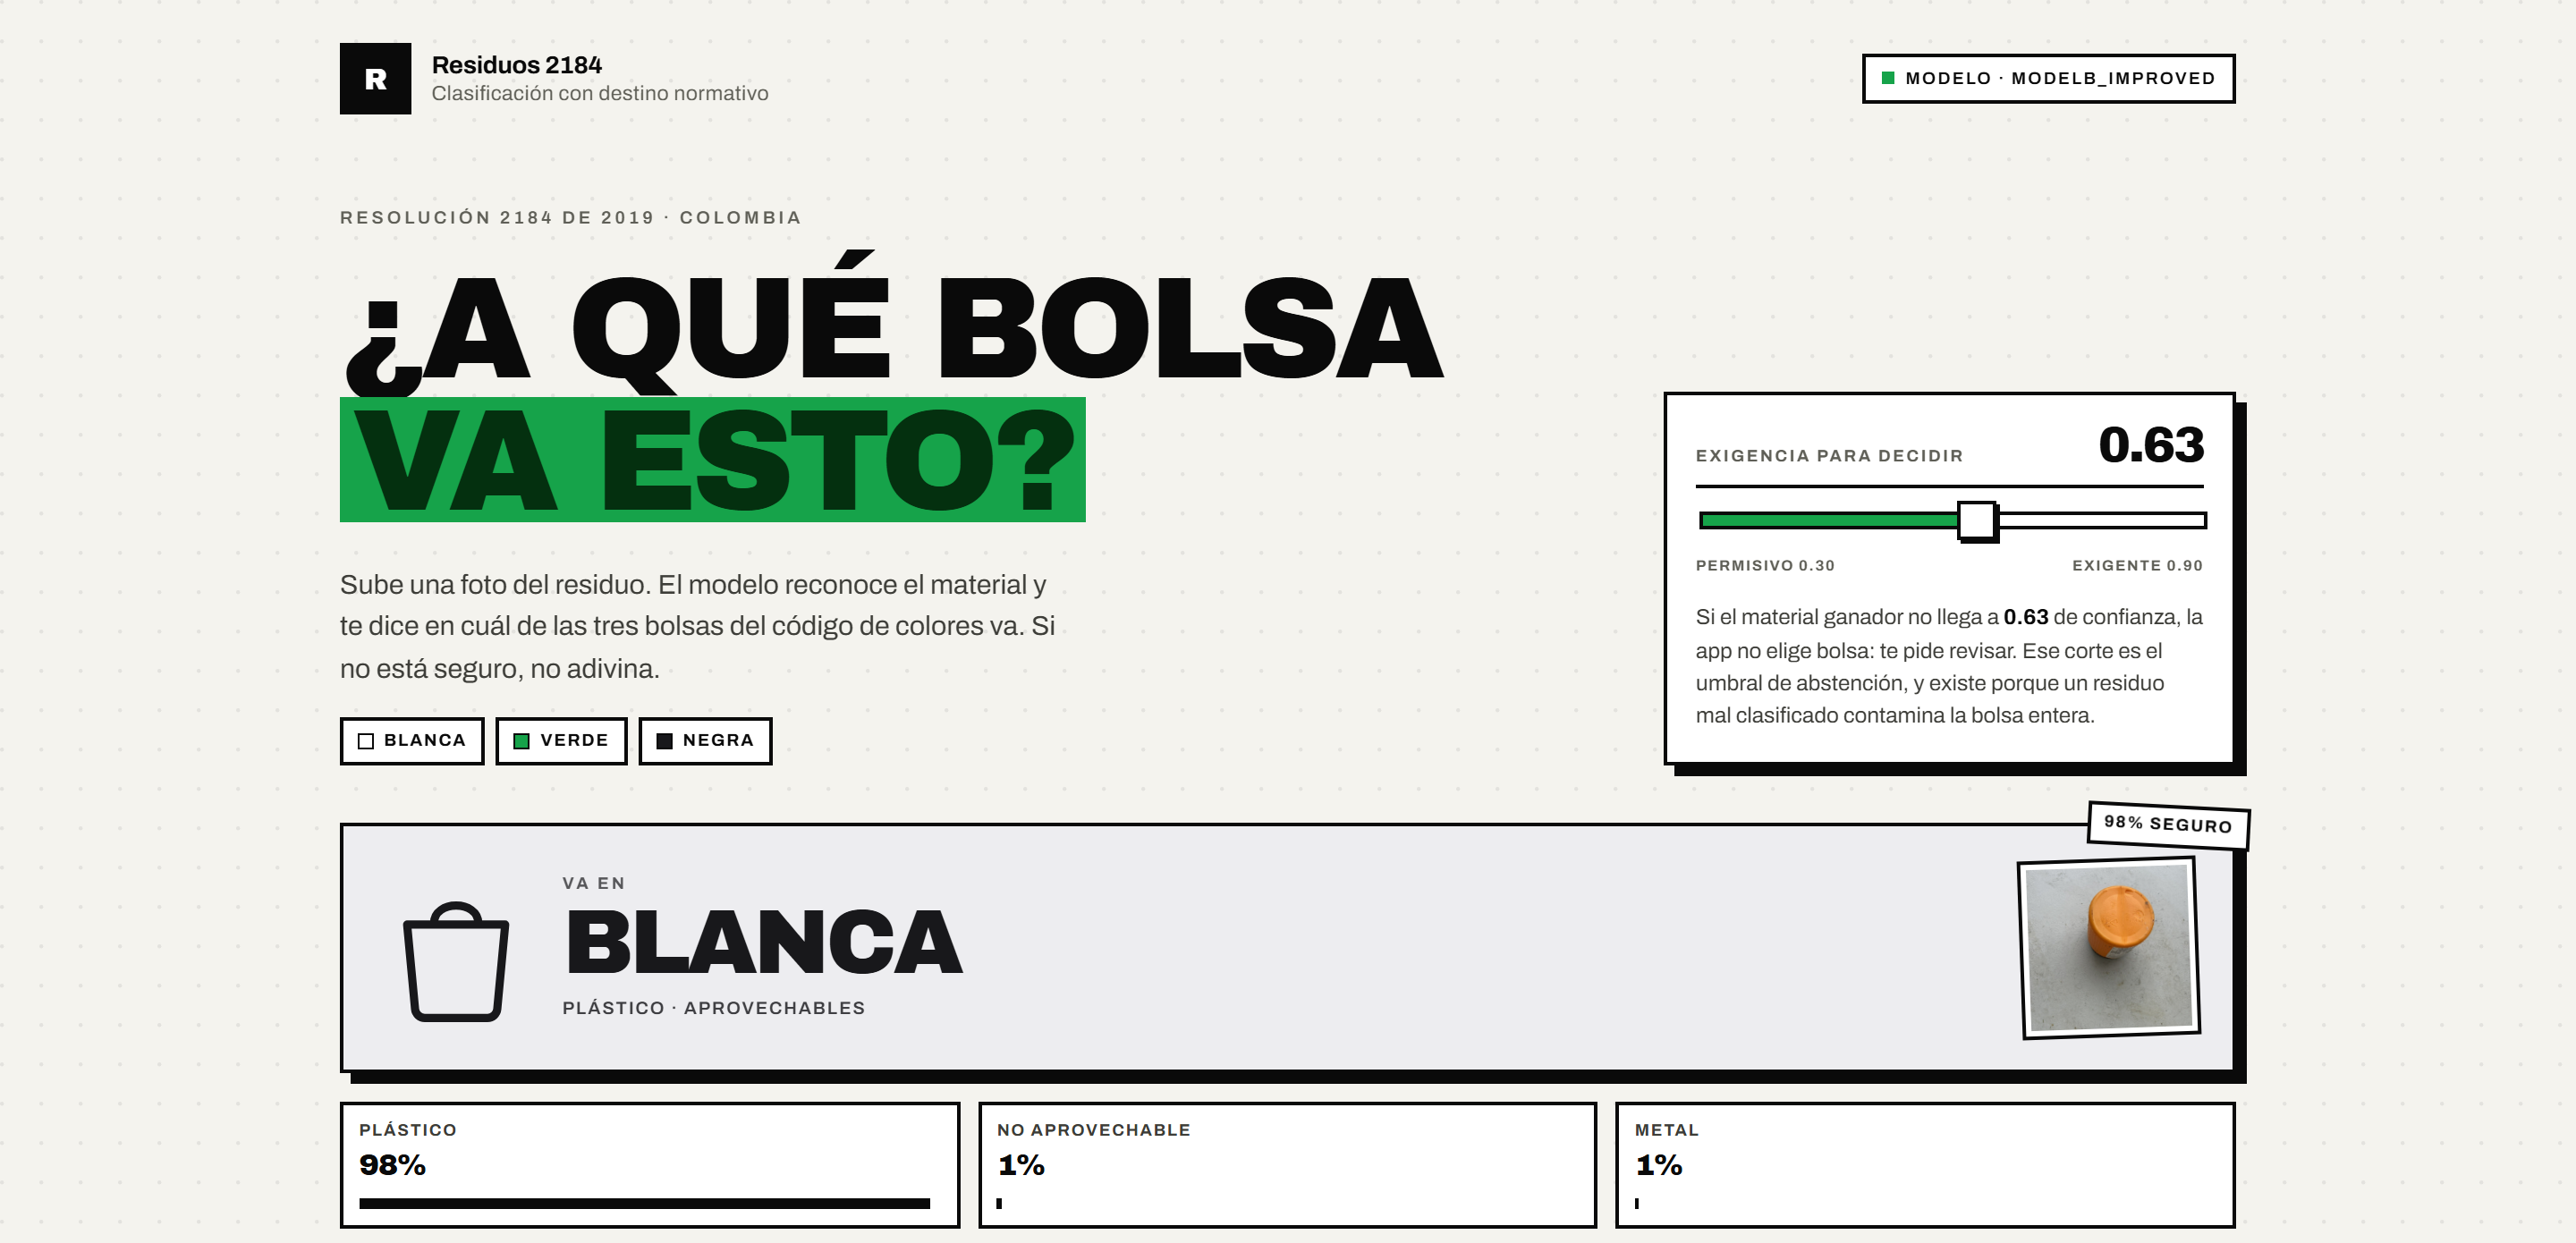
\includegraphics[width=0.92\textwidth]{ui_veredicto.png}
\caption{Interfaz con una foto: material, bolsa, confianza y top-3.}
\label{fig:ui_veredicto}
\end{figure*}

\begin{figure*}[t]
\centering
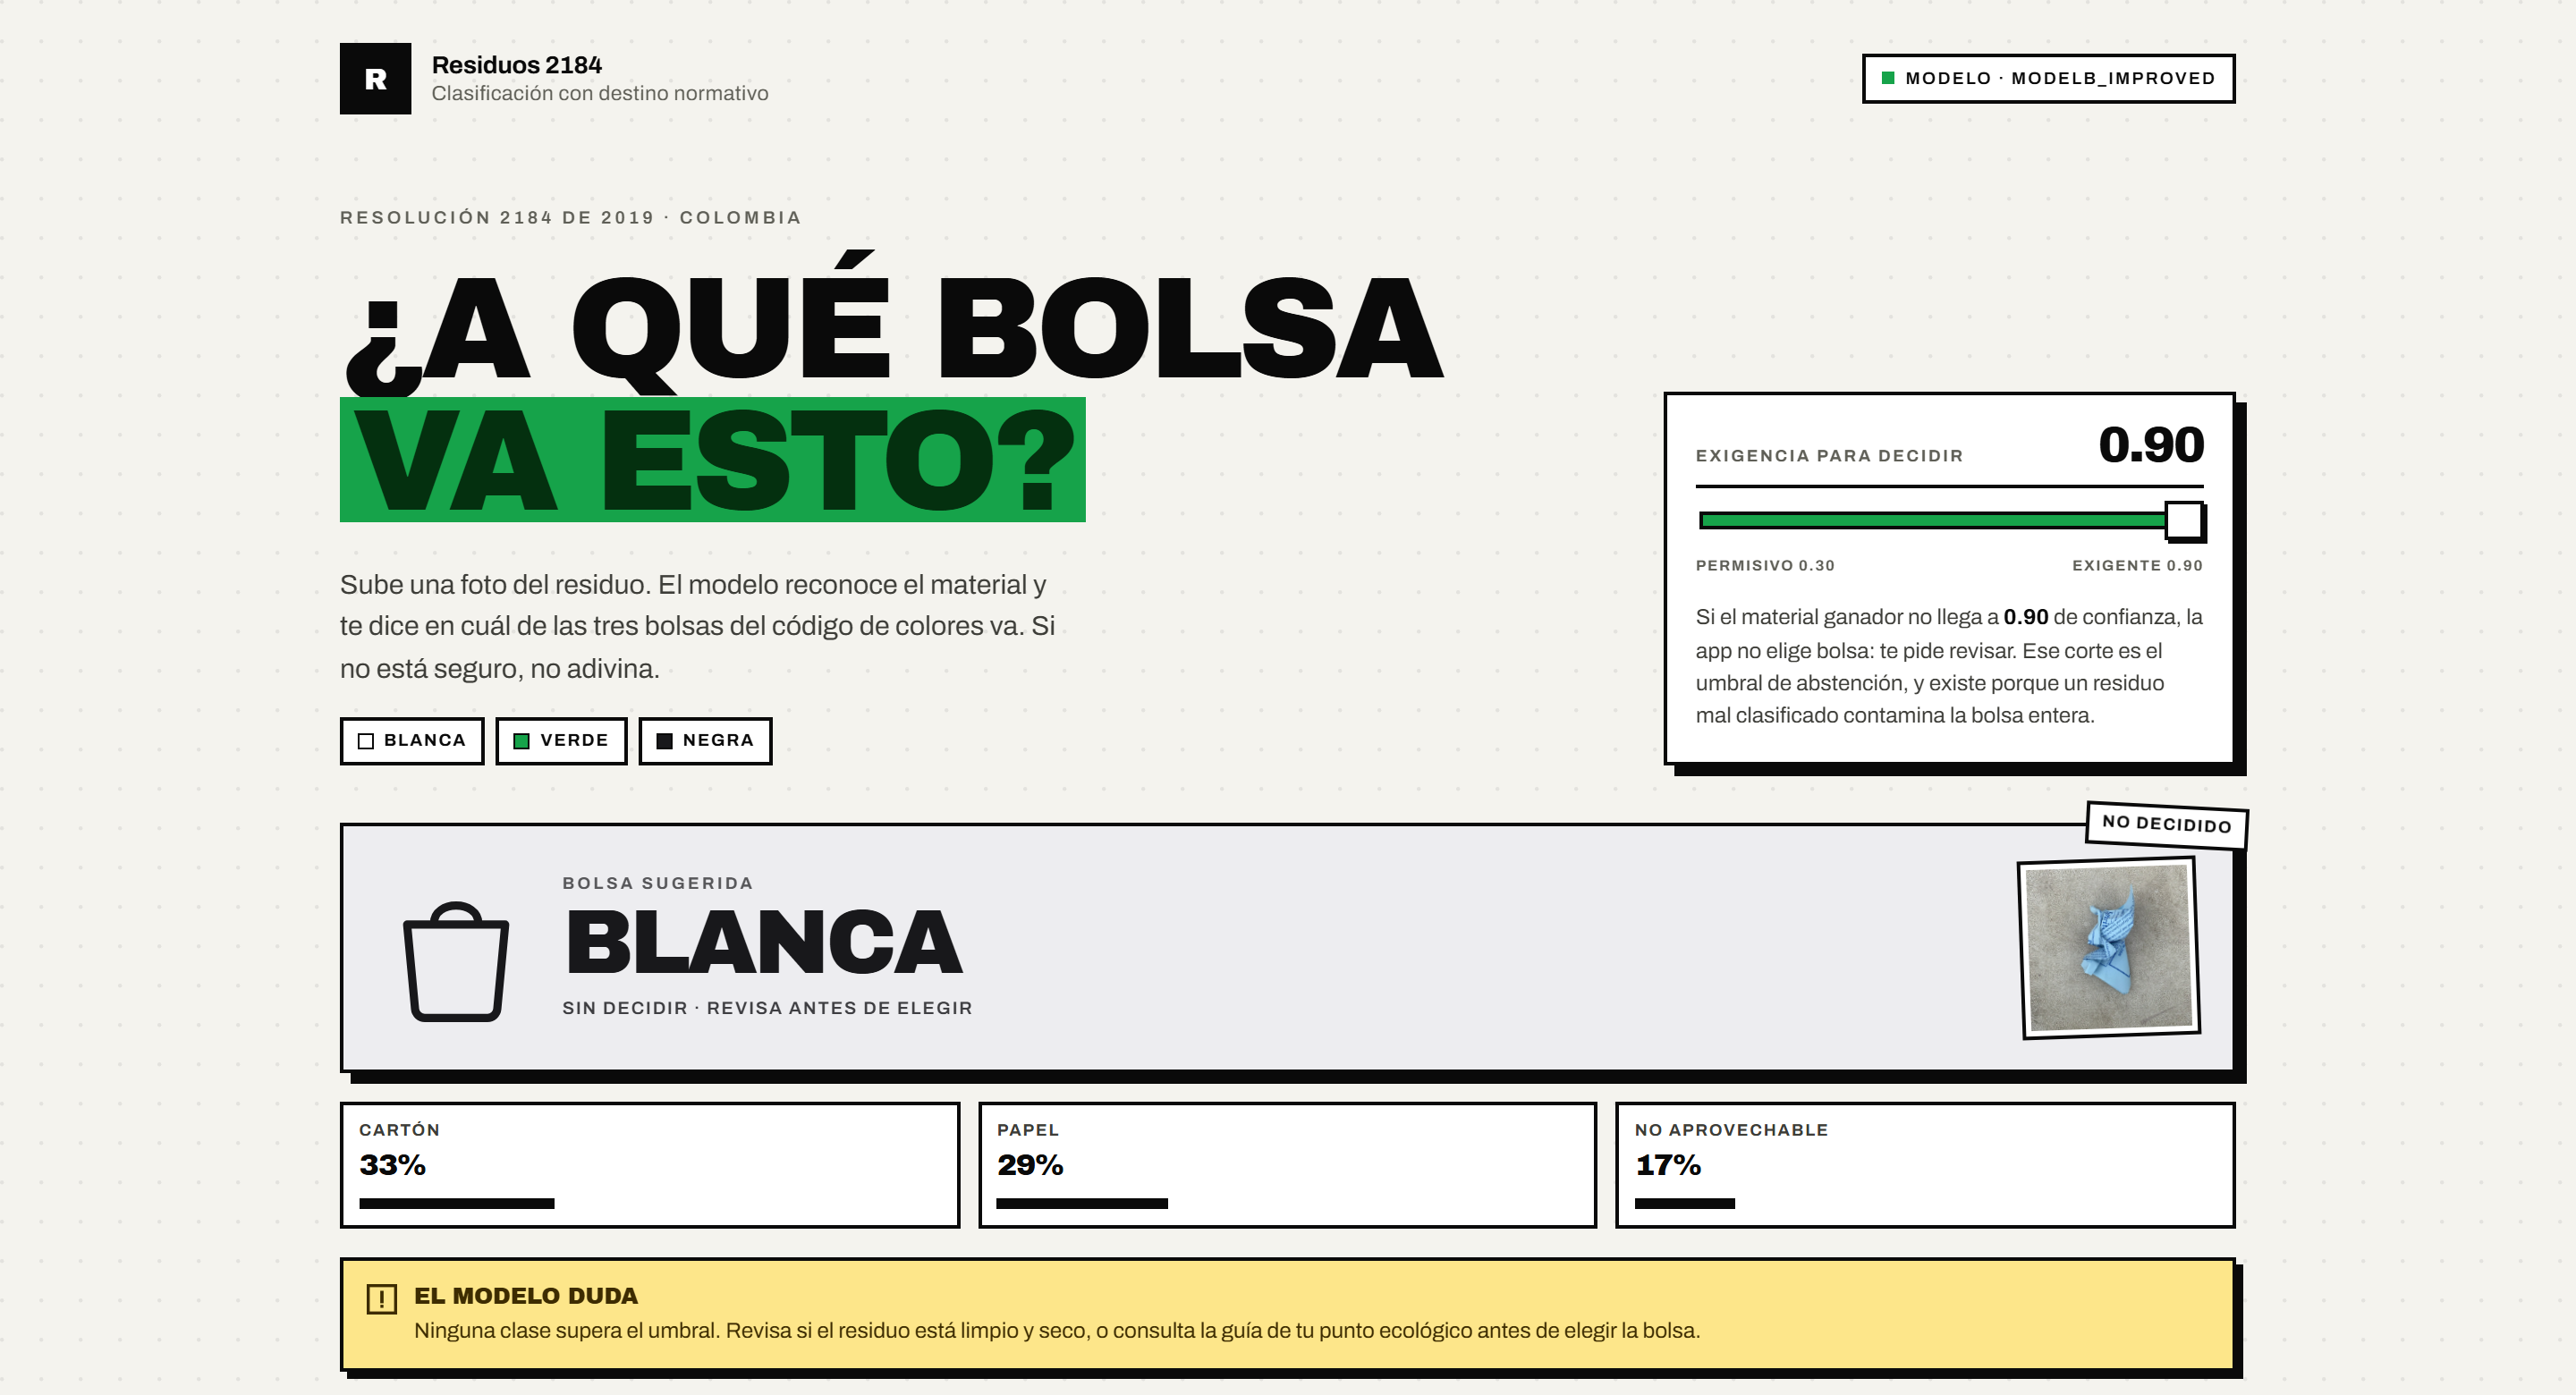
\includegraphics[width=0.92\textwidth]{ui_abstencion.png}
\caption{Abstenci\'on con el umbral en 0,90: la aplicaci\'on pide revisar en
lugar de adivinar.}
\label{fig:ui_abstencion}
\end{figure*}

\begin{figure*}[t]
\centering
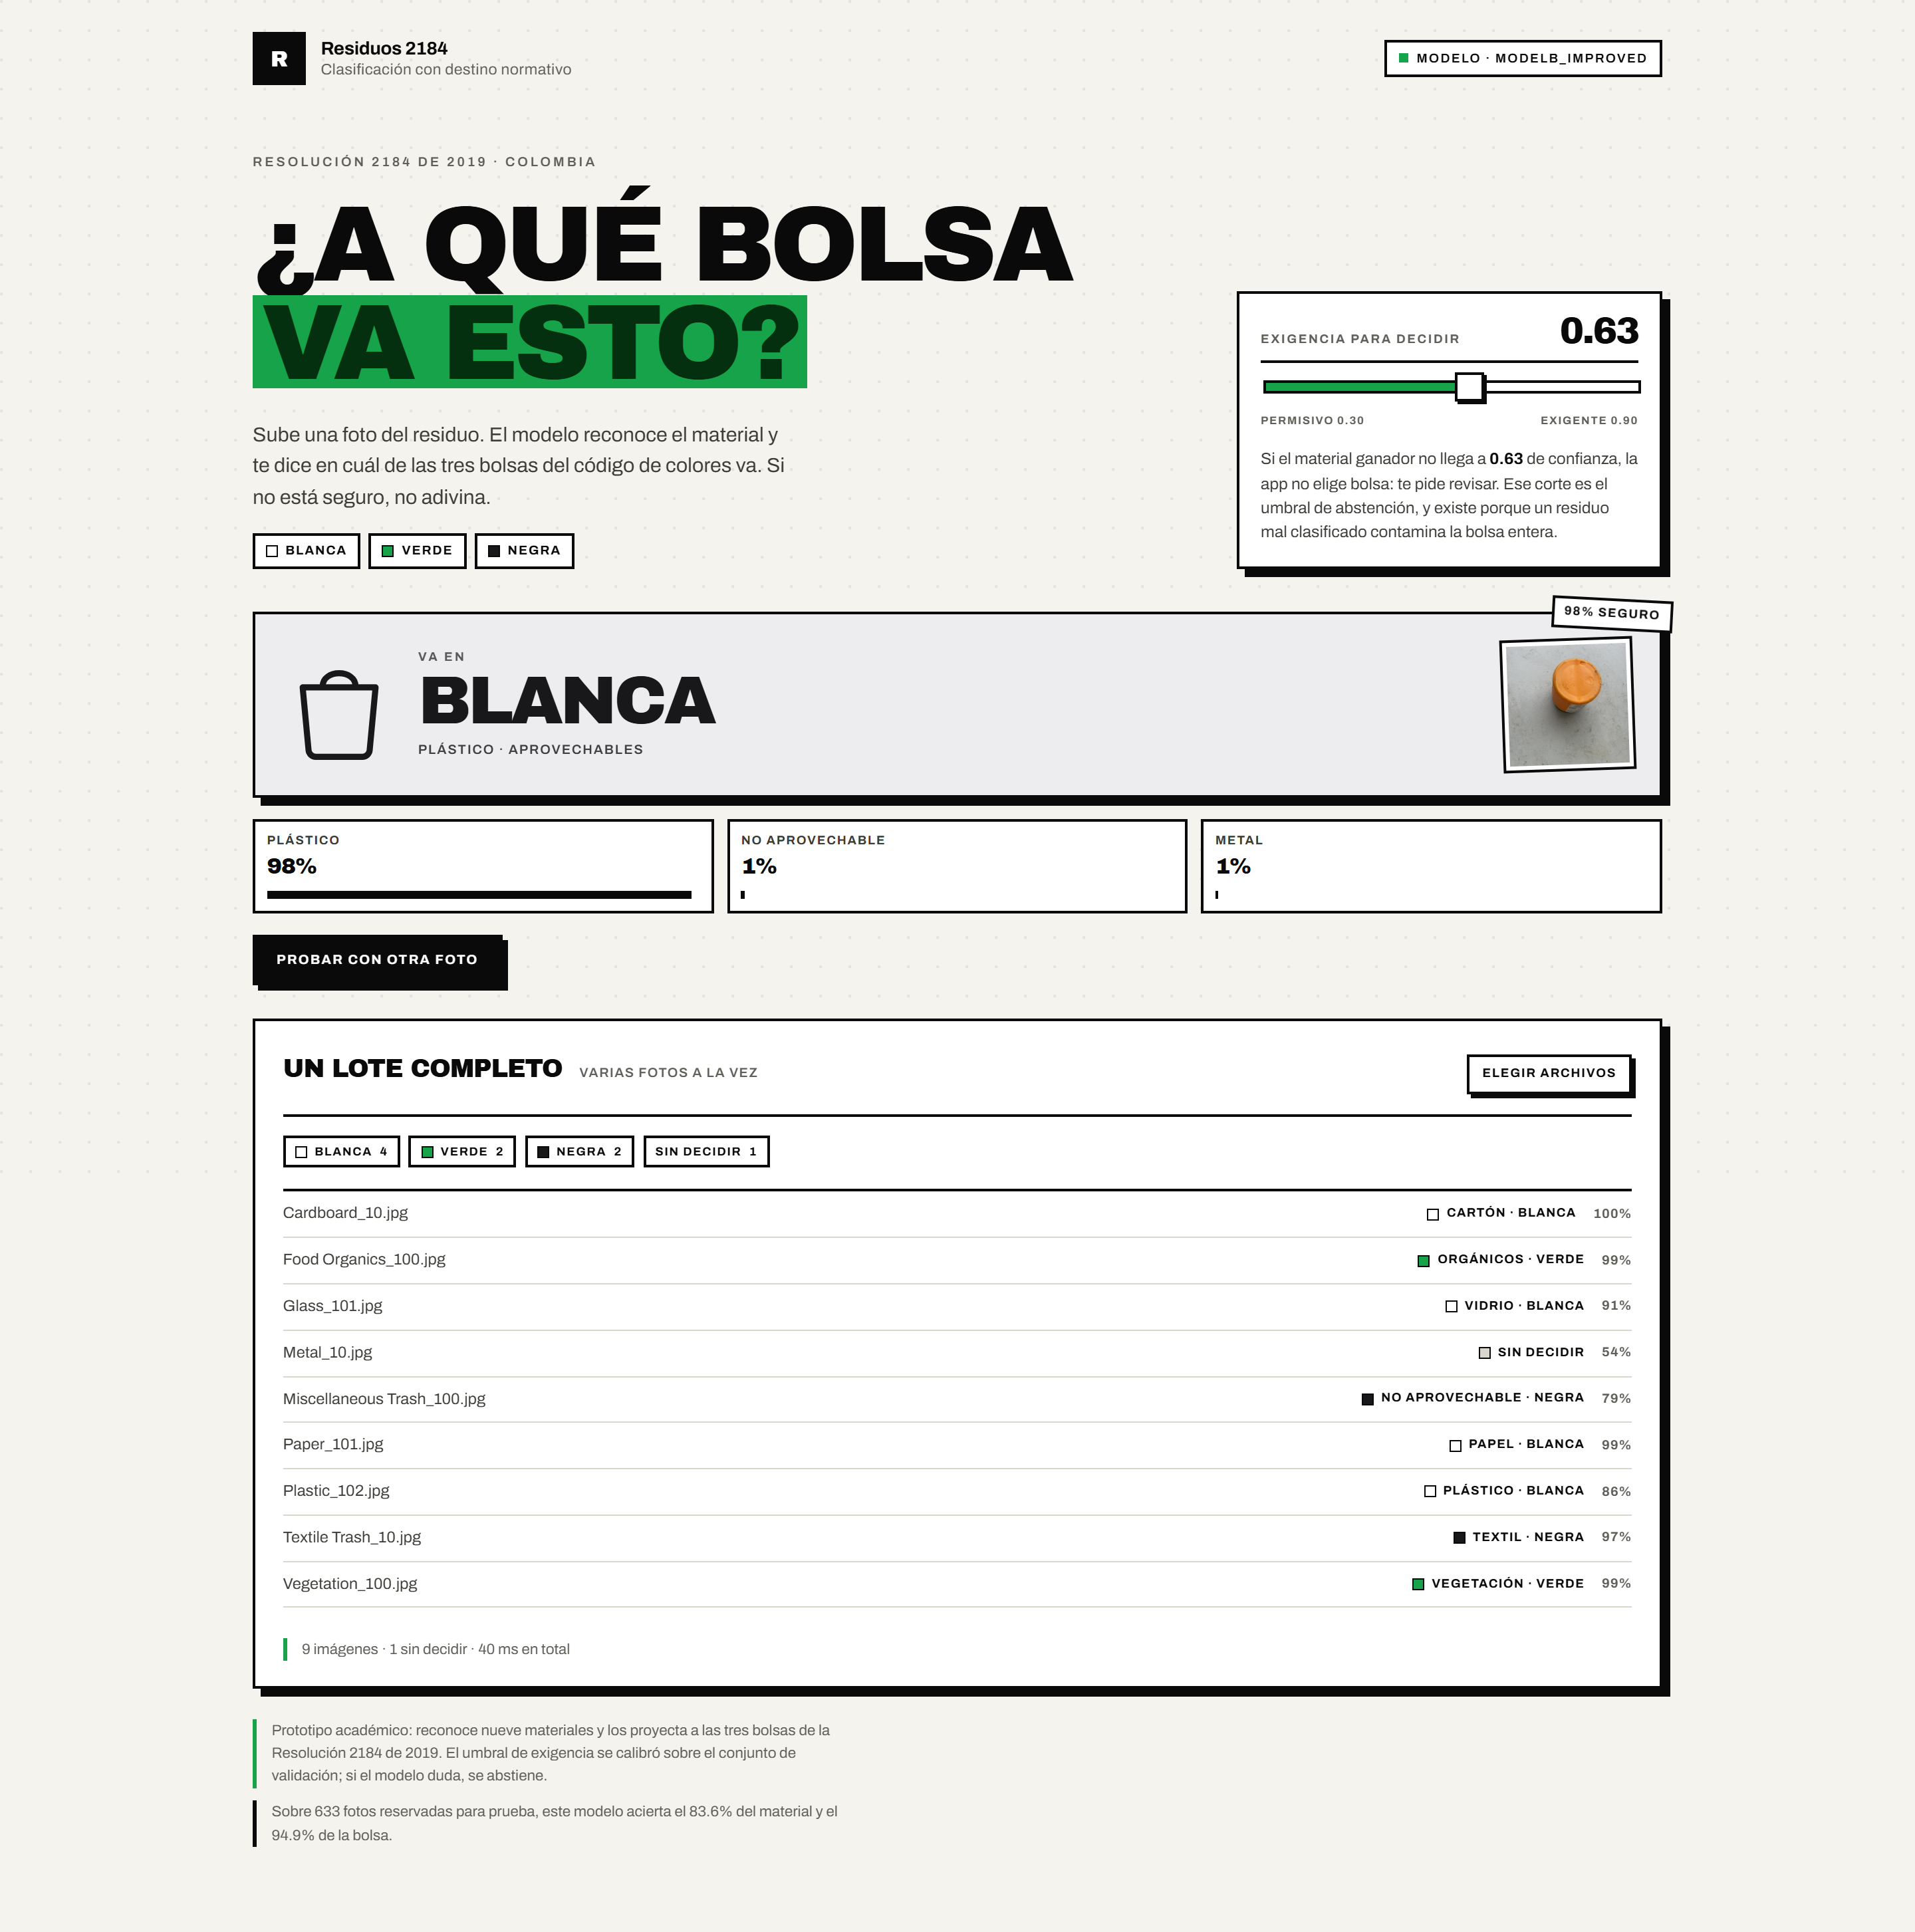
\includegraphics[width=0.86\textwidth]{ui_lote.png}
\caption{Vista de lote: cada foto con su decisi\'on y el resumen por bolsa.}
\label{fig:ui_lote}
\end{figure*}

\begin{figure}[!b]
\centering
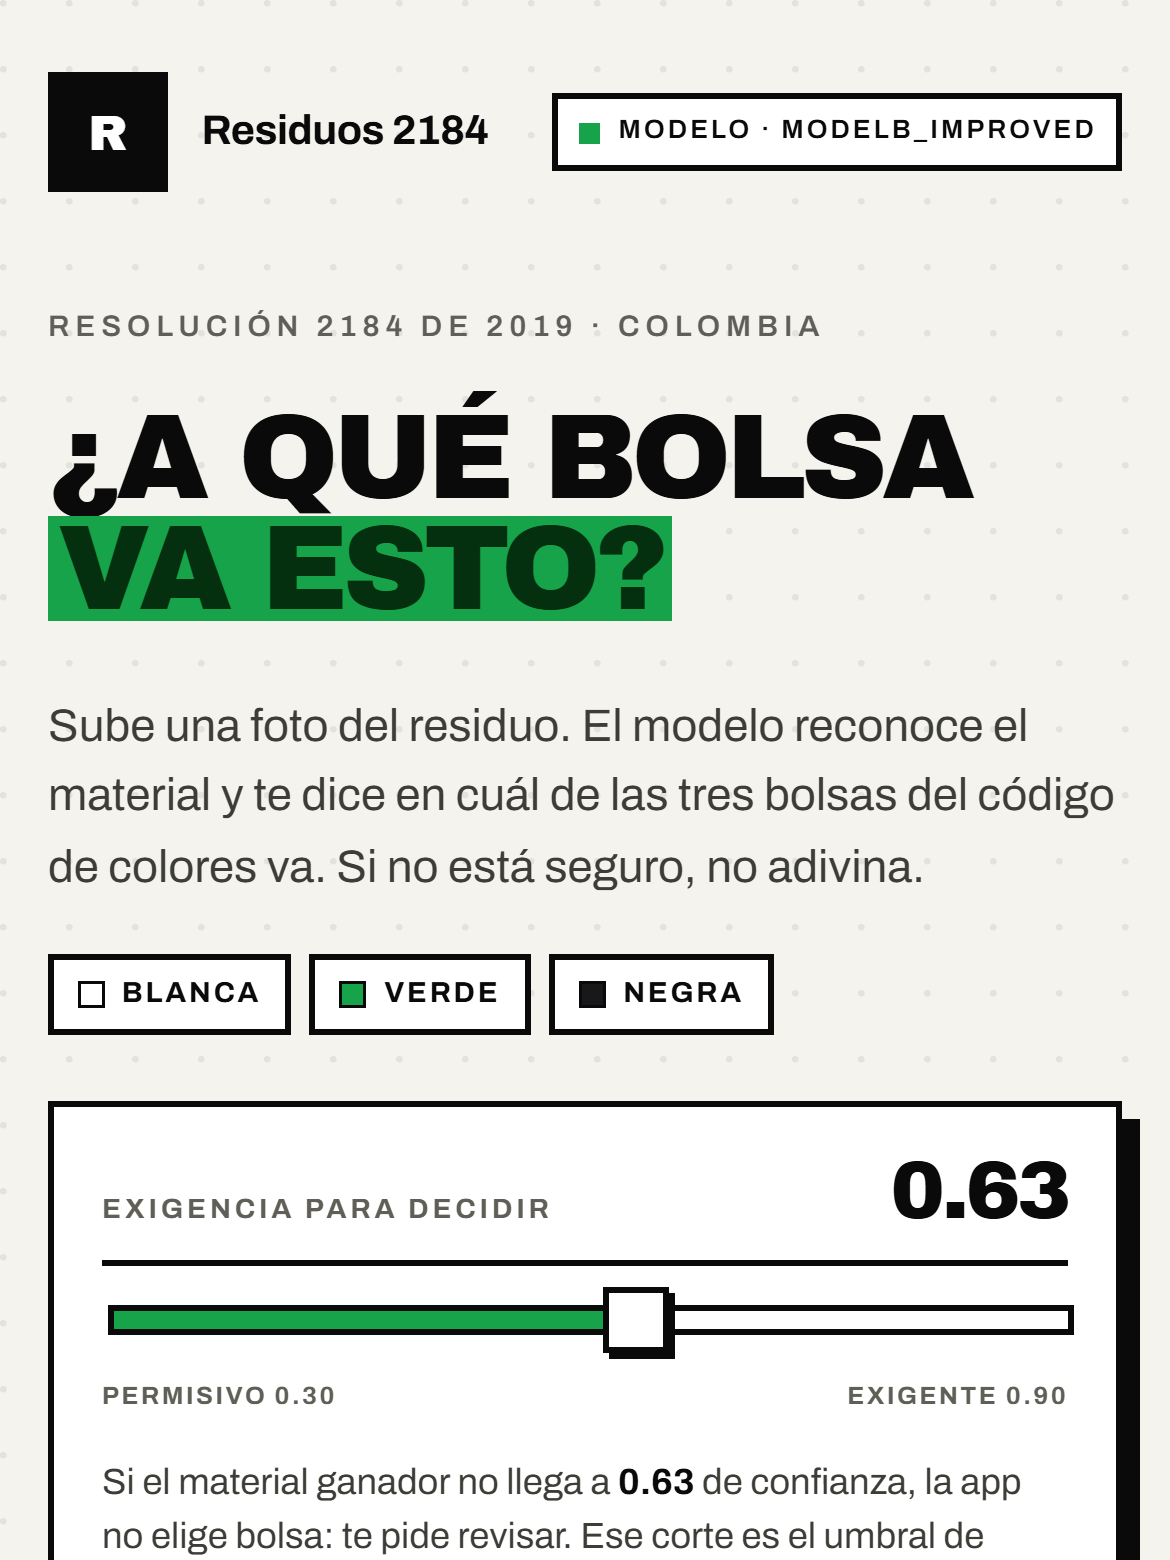
\includegraphics[width=0.64\columnwidth]{ui_movil.png}
\caption{Vista m\'ovil de la aplicaci\'on en producci\'on.}
\label{fig:ui_movil}
\end{figure}

\subsection{Pruebas}

El repositorio tiene 35 pruebas automatizadas en cuatro suites. La suite de datos
verifica la huella dHash, la deduplicaci\'on, la estratificaci\'on y la
reproducibilidad de la partici\'on. La de dominio cubre la proyecci\'on a bolsas,
la conservaci\'on de la masa de probabilidad, la abstenci\'on, el car\'acter
inclusivo del umbral y el top-3. La de imagen comprueba la forma NHWC, el rango
$[-1,1]$, el orden RGB y la escala de grises. La de inferencia cubre el doble
softmax y el contrato HTTP, incluidos los lotes y los archivos inv\'alidos. Las 35
pruebas corren en menos de un segundo y son el primer paso del pipeline.

\subsection{Despliegue y CI/CD}

La imagen se construye en dos etapas: una imagen de Rust compila el WASM con
\texttt{trunk} y una imagen \texttt{python:3.12-slim} instala las dependencias,
copia la API, los modelos y el WASM, crea un usuario sin privilegios y declara un
\texttt{HEALTHCHECK} contra \texttt{/api/health}. La imagen final pesa
aproximadamente 471 MB y no publica puertos.

En el VPS, Traefik termina TLS con Let's Encrypt y enruta el dominio a la red
interna \texttt{web}; el contenedor solo es alcanzable por esa red. El archivo
\texttt{.env} se materializa desde OpenBao y el tag desplegado se guarda en
\texttt{.release.env}, de modo que un \texttt{docker compose up -d} posterior no
vuelve a \texttt{:latest}. El despliegue lo ejecuta un usuario
\texttt{deploy-residuos} con \texttt{ForceCommand}: solo puede invocar
\texttt{residuos-deploy <tag>}, y el wrapper valida el tag contra una allowlist.
El CI corre las pruebas, escanea secretos con gitleaks y publica la imagen en
GHCR; el despliegue se dispara con un tag \texttt{vX.Y.Z} o con una ejecuci\'on
manual que indica el tag. Como el puerto SSH p\'ublico est\'a cerrado, el runner
entra por un nodo ef\'imero de Tailscale. La Fig.~\ref{fig:ci} muestra una
ejecuci\'on completa: pruebas, imagen y despliegue en verde.

\begin{figure*}[t]
\centering
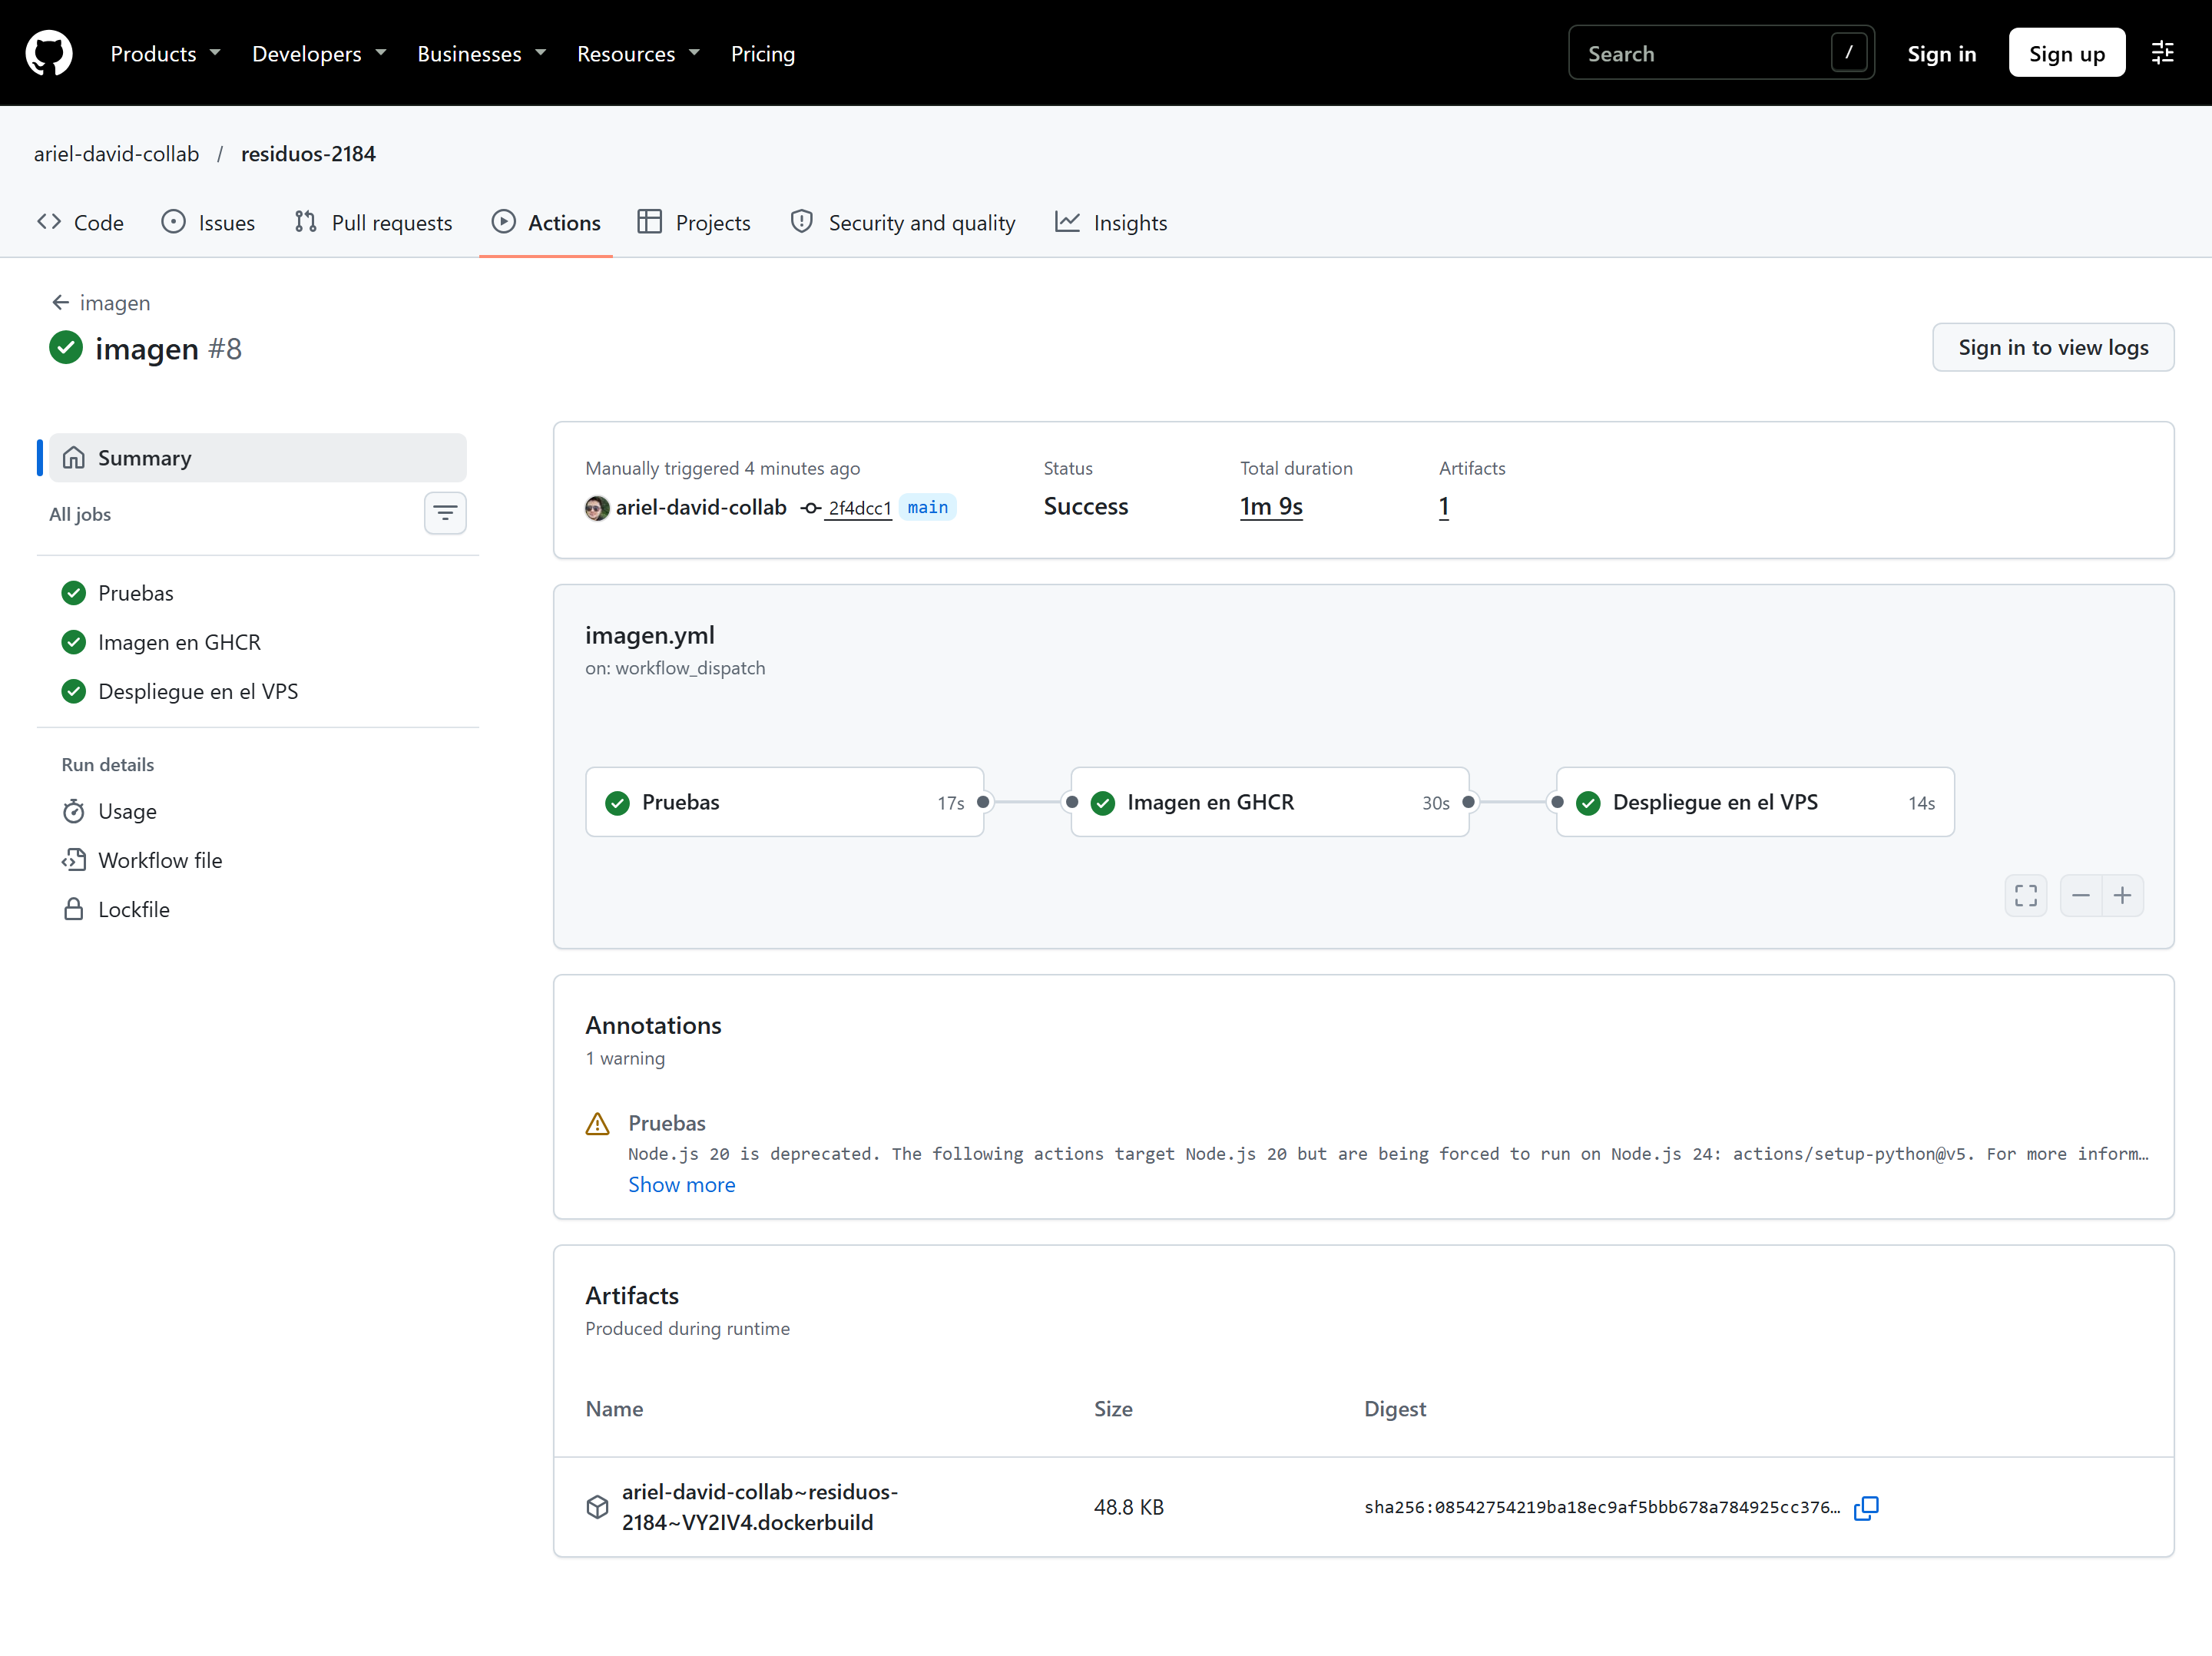
\includegraphics[width=0.82\textwidth]{ci_run.png}
\caption{Ejecuci\'on del pipeline: pruebas (17 s), imagen en GHCR (30 s) y
despliegue en el VPS (14 s).}
\label{fig:ci}
\end{figure*}

\subsection{Reproducibilidad}

Los scripts \texttt{s01} a \texttt{s06} reproducen el material del informe:
inventario y partici\'on, figuras exploratorias, entrenamiento del Modelo A,
conversi\'on a ONNX, entrenamiento del Modelo B, calibraci\'on y evaluaci\'on. Las
figuras y las capturas se generan con programas del repositorio, no con capturas
manuales de ventanas; cada PNG tiene al lado el archivo de texto o el script que
lo produjo. El Ap\'endice~\ref{app:repro} lista los comandos.

\subsection{Seguridad y operaci\'on}

El contenedor corre como usuario sin privilegios y no publica puertos: solo lo
alcanza Traefik por la red interna \texttt{web}, que es el \'unico punto de
entrada y el que termina TLS. Las credenciales no viven en el repositorio; el
archivo \texttt{.env} se materializa desde OpenBao y el tag desplegado queda
registrado en \texttt{.release.env}. El usuario de despliegue tiene un
\texttt{ForceCommand} que solo acepta \texttt{residuos-deploy <tag>} y valida el
tag contra una allowlist, de modo que una llave comprometida no entrega una
shell. En el CI, gitleaks escanea cada push y la imagen solo se publica si las
pruebas pasan; el despliegue autom\'atico se limita a tags \texttt{vX.Y.Z} y una
ejecuci\'on manual debe indicar el tag de forma expl\'icita. El runner no abre el
puerto SSH: entra por un nodo ef\'imero de Tailscale. La aplicaci\'on no
almacena las fotos y la respuesta incluye solo el veredicto, las probabilidades
y la latencia.

% ============================================================================
\section{Resultados}
\label{sec:resultados}
\label{sec:resultados}

\subsection{Comparaci\'on global}

La Tabla~\ref{tab:global} resume la evaluaci\'on sobre las 633 im\'agenes de
\texttt{test/}. El Modelo B supera al A en todas las m\'etricas: +5,4 puntos de
exactitud de material, +3,0 de exactitud de bolsa, +0,064 de F1 macro y +0,017 de
AUC. La diferencia m\'as grande est\'a en el log-loss: 0,450 frente a 0,976, lo
que indica que las probabilidades del B son mucho m\'as informativas. Esa
propiedad es la que hace \'util la abstenci\'on: un modelo sobreconfiado no puede
callar de forma selectiva.

\begin{table*}[t]
\centering
\caption{Resultados sobre \texttt{test/} (633 im\'agenes). Mejor valor en negrita.}
\label{tab:global}
\footnotesize
\setlength{\tabcolsep}{6pt}
\begin{tabular}{@{}lrrrrrrr@{}}
\toprule
Modelo & Exactitud & Top-2 & Log-loss & F1 macro & AUC macro & Bolsa & F1 bolsa \\
\midrule
A (Teachable Machine) & 0,782 & 0,904 & 0,976 & 0,777 & 0,971 & 0,919 & 0,889 \\
B (MobileNetV3-Small) & \textbf{0,836} & \textbf{0,951} & \textbf{0,450} &
\textbf{0,841} & \textbf{0,987} & \textbf{0,949} & \textbf{0,931} \\
\bottomrule
\end{tabular}
\end{table*}

\subsection{Comportamiento por clase}

La Tabla~\ref{tab:clases} desglosa el Modelo B. Las clases con mejor F1 son
Vegetaci\'on (0,968), Vidrio (0,891) y Org\'anicos (0,889); las peores son No
aprovechable (0,746), Textil (0,777) y Pl\'astico (0,788). El caso del Pl\'astico
es el m\'as instructivo: tiene la mayor precisi\'on de su grupo (0,881) pero el
recall m\'as bajo (0,712), porque 18 de sus 125 im\'agenes se predicen como
Metal. El modelo es conservador con el pl\'astico: cuando lo declara, acierta; lo
que falla es reconocerlo en todas sus formas.

\begin{table}[t]
\centering
\caption{Modelo B por clase en \texttt{test/}: precisi\'on, recall, F1 y AUC.
La \'ultima columna compara el F1 del Modelo A.}
\label{tab:clases}
\footnotesize
\setlength{\tabcolsep}{2.8pt}
\begin{tabular}{@{}lrrrrr@{}}
\toprule
Clase & P & R & F1 & AUC & F1$_A$ \\
\midrule
Cart\'on        & 0,831 & 0,831 & 0,831 & 0,980 & 0,756 \\
Org\'anicos     & 0,836 & 0,949 & 0,889 & 0,997 & 0,867 \\
Vidrio          & 0,845 & 0,942 & 0,891 & 0,997 & 0,737 \\
Metal           & 0,741 & 0,870 & 0,800 & 0,981 & 0,794 \\
No aprovechable & 0,771 & 0,723 & 0,746 & 0,976 & 0,641 \\
Papel           & 0,882 & 0,870 & 0,876 & 0,990 & 0,750 \\
Pl\'astico      & 0,881 & 0,712 & 0,788 & 0,970 & 0,807 \\
Textil          & 0,767 & 0,786 & 0,777 & 0,992 & 0,702 \\
Vegetaci\'on    & 0,984 & 0,953 & 0,968 & 1,000 & 0,939 \\
\bottomrule
\end{tabular}
\end{table}

\subsection{Matrices de confusi\'on}

La Fig.~\ref{fig:matriz_mat} compara las matrices de materiales de los dos
modelos. La diagonal del B es m\'as limpia, sobre todo en Org\'anicos, Vidrio y
Vegetaci\'on. Los errores del B se concentran en la frontera Pl\'astico--Metal
(18 casos) y en la confusi\'on de No aprovechable con Textil (5) y Metal (5). El
A, en cambio, dispersa m\'as: confunde Cart\'on con Papel (7), Vidrio con
Pl\'astico (9) y No aprovechable con Textil (8). Esa dispersi\'on explica su peor
F1 macro aunque su exactitud no sea muy inferior.

\begin{figure*}[!t]
\centering
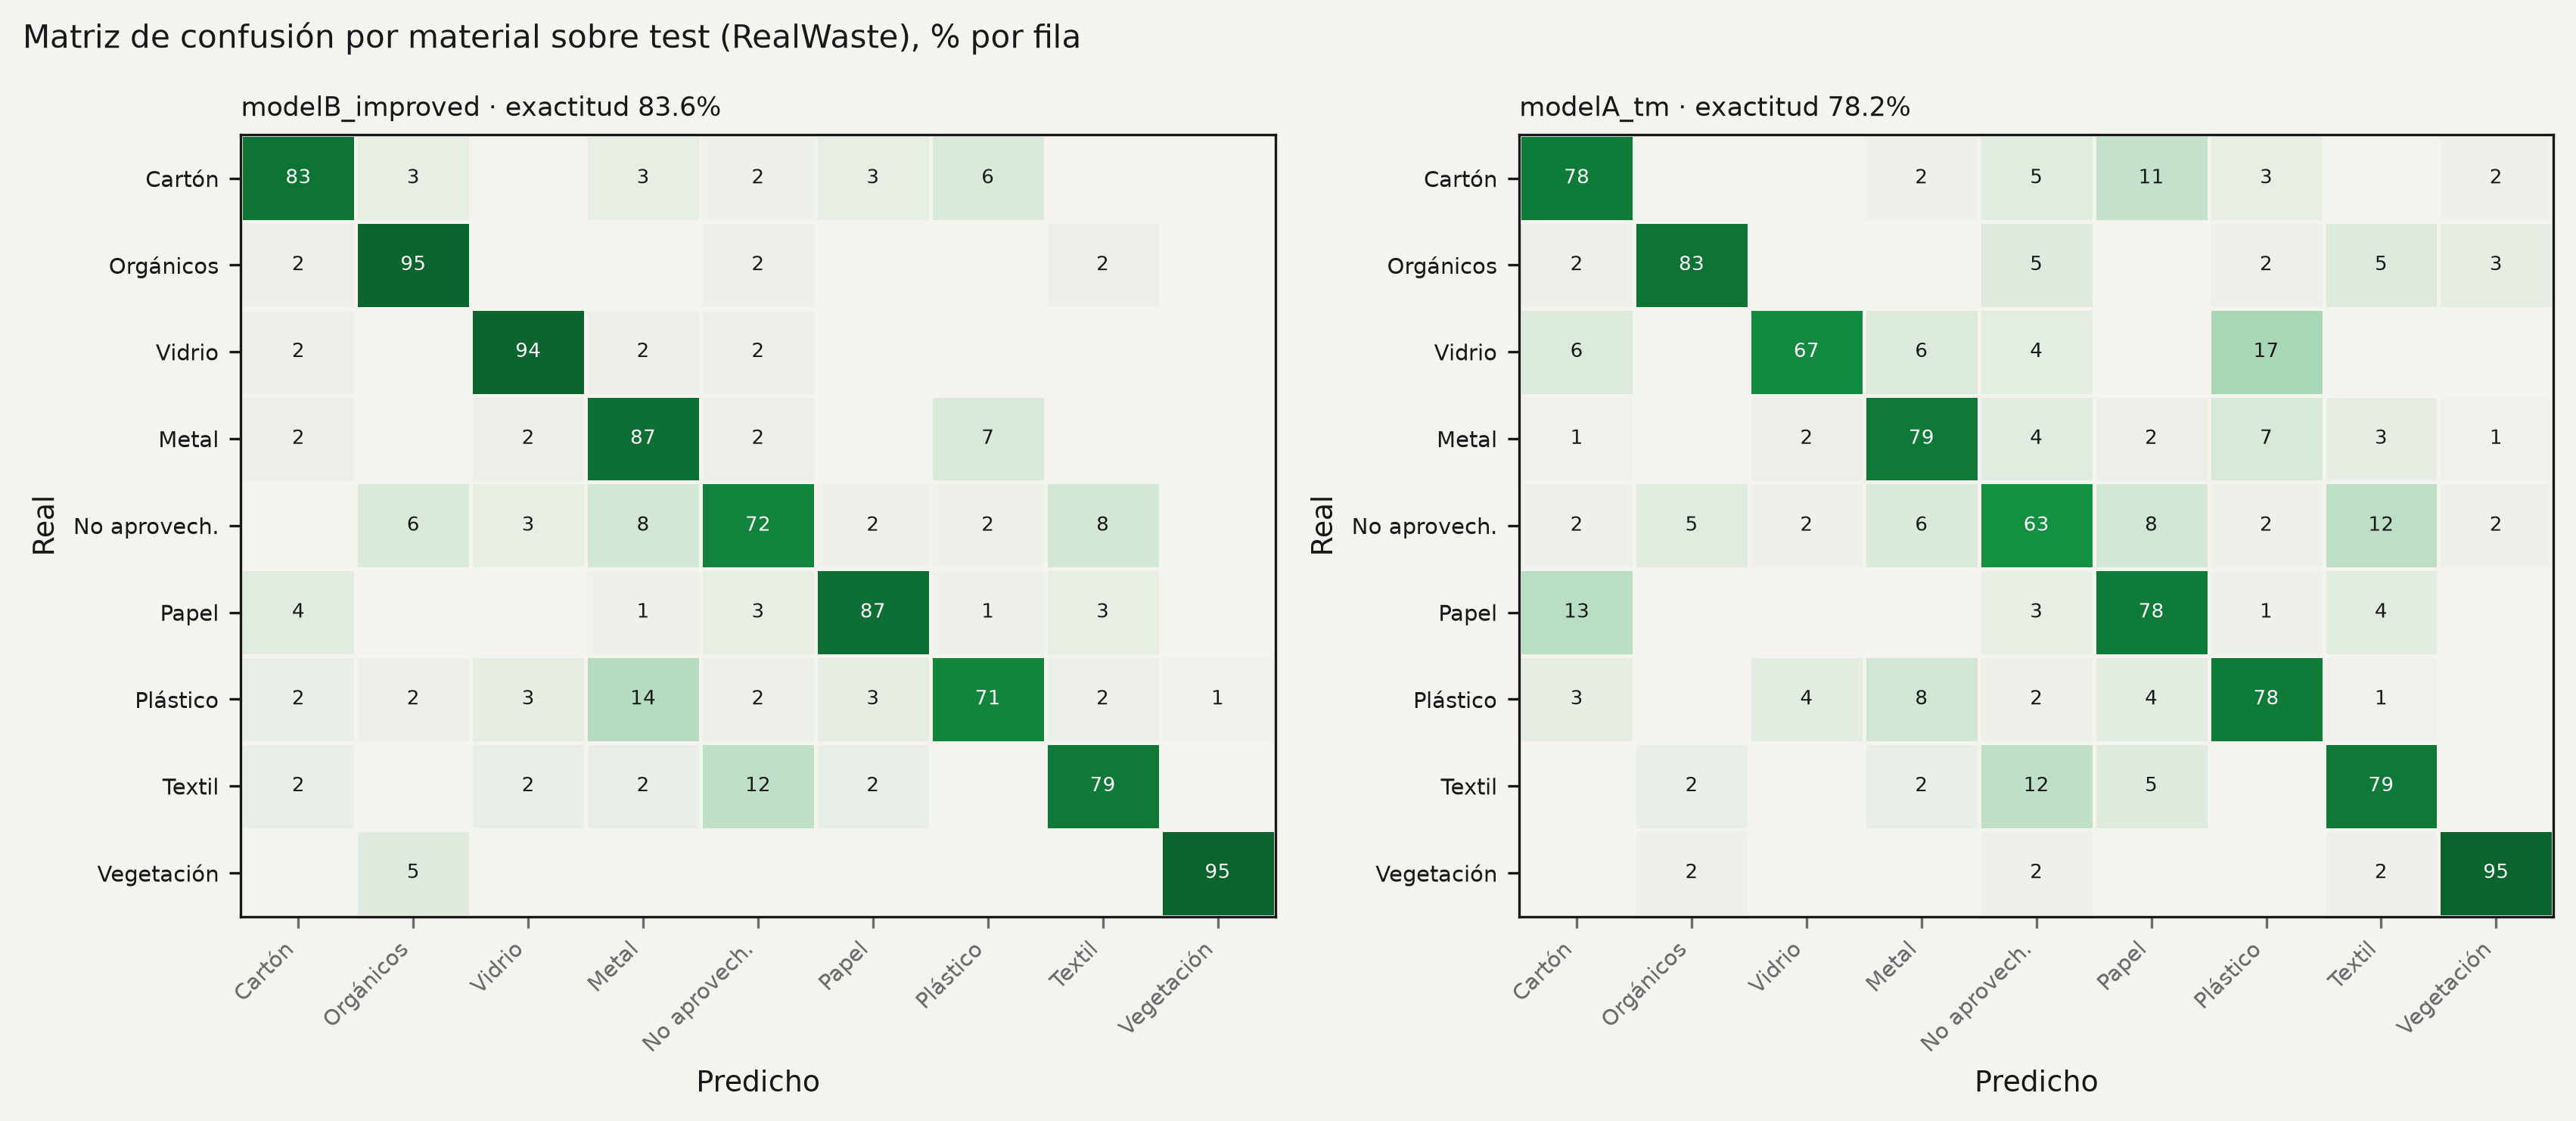
\includegraphics[width=0.9\textwidth]{matriz_materiales.png}
\caption{Matrices de confusi\'on de materiales: Modelo A (izquierda) y Modelo B
(derecha).}
\label{fig:matriz_mat}
\end{figure*}

\subsection{Decisi\'on de bolsa}

La Tabla~\ref{tab:bolsas} y la Fig.~\ref{fig:matriz_bolsas} muestran el nivel que
realmente importa. El Modelo B acierta el 94,9\,\% de las bolsas; la blanca, con
403 casos, alcanza 0,968 de F1; la verde, 0,952; la negra, 0,873. La bolsa negra
es la m\'as dif\'icil: 18 de sus 107 casos se predicen como blanca o verde. El
Modelo A baja a 0,919 y su bolsa negra cae a 0,785, lastrada por 21 casos que se
van a la blanca. La diferencia entre modelos es menor a nivel de bolsa que a nivel
de material, justamente porque la proyecci\'on agrupa cinco materiales en la
blanca y perdona errores entre ellos.

\begin{table}[t]
\centering
\caption{Resultados por bolsa en \texttt{test/}.}
\label{tab:bolsas}
\footnotesize
\setlength{\tabcolsep}{4pt}
\begin{tabular}{@{}lrrrrrr@{}}
\toprule
 & & \multicolumn{3}{c}{Modelo B} & \multicolumn{2}{c}{Modelo A} \\
\cmidrule(lr){3-5}\cmidrule(lr){6-7}
Bolsa & Sop. & P & R & F1 & R & F1 \\
\midrule
Blanca & 403 & 0,963 & 0,973 & 0,968 & 0,950 & 0,953 \\
Verde  & 123 & 0,930 & 0,976 & 0,952 & 0,919 & 0,930 \\
Negra  & 107 & 0,918 & 0,832 & 0,873 & 0,804 & 0,785 \\
\midrule
Global & 633 & -- & -- & 0,931 & -- & 0,889 \\
\bottomrule
\end{tabular}
\end{table}

\begin{figure*}[!t]
\centering
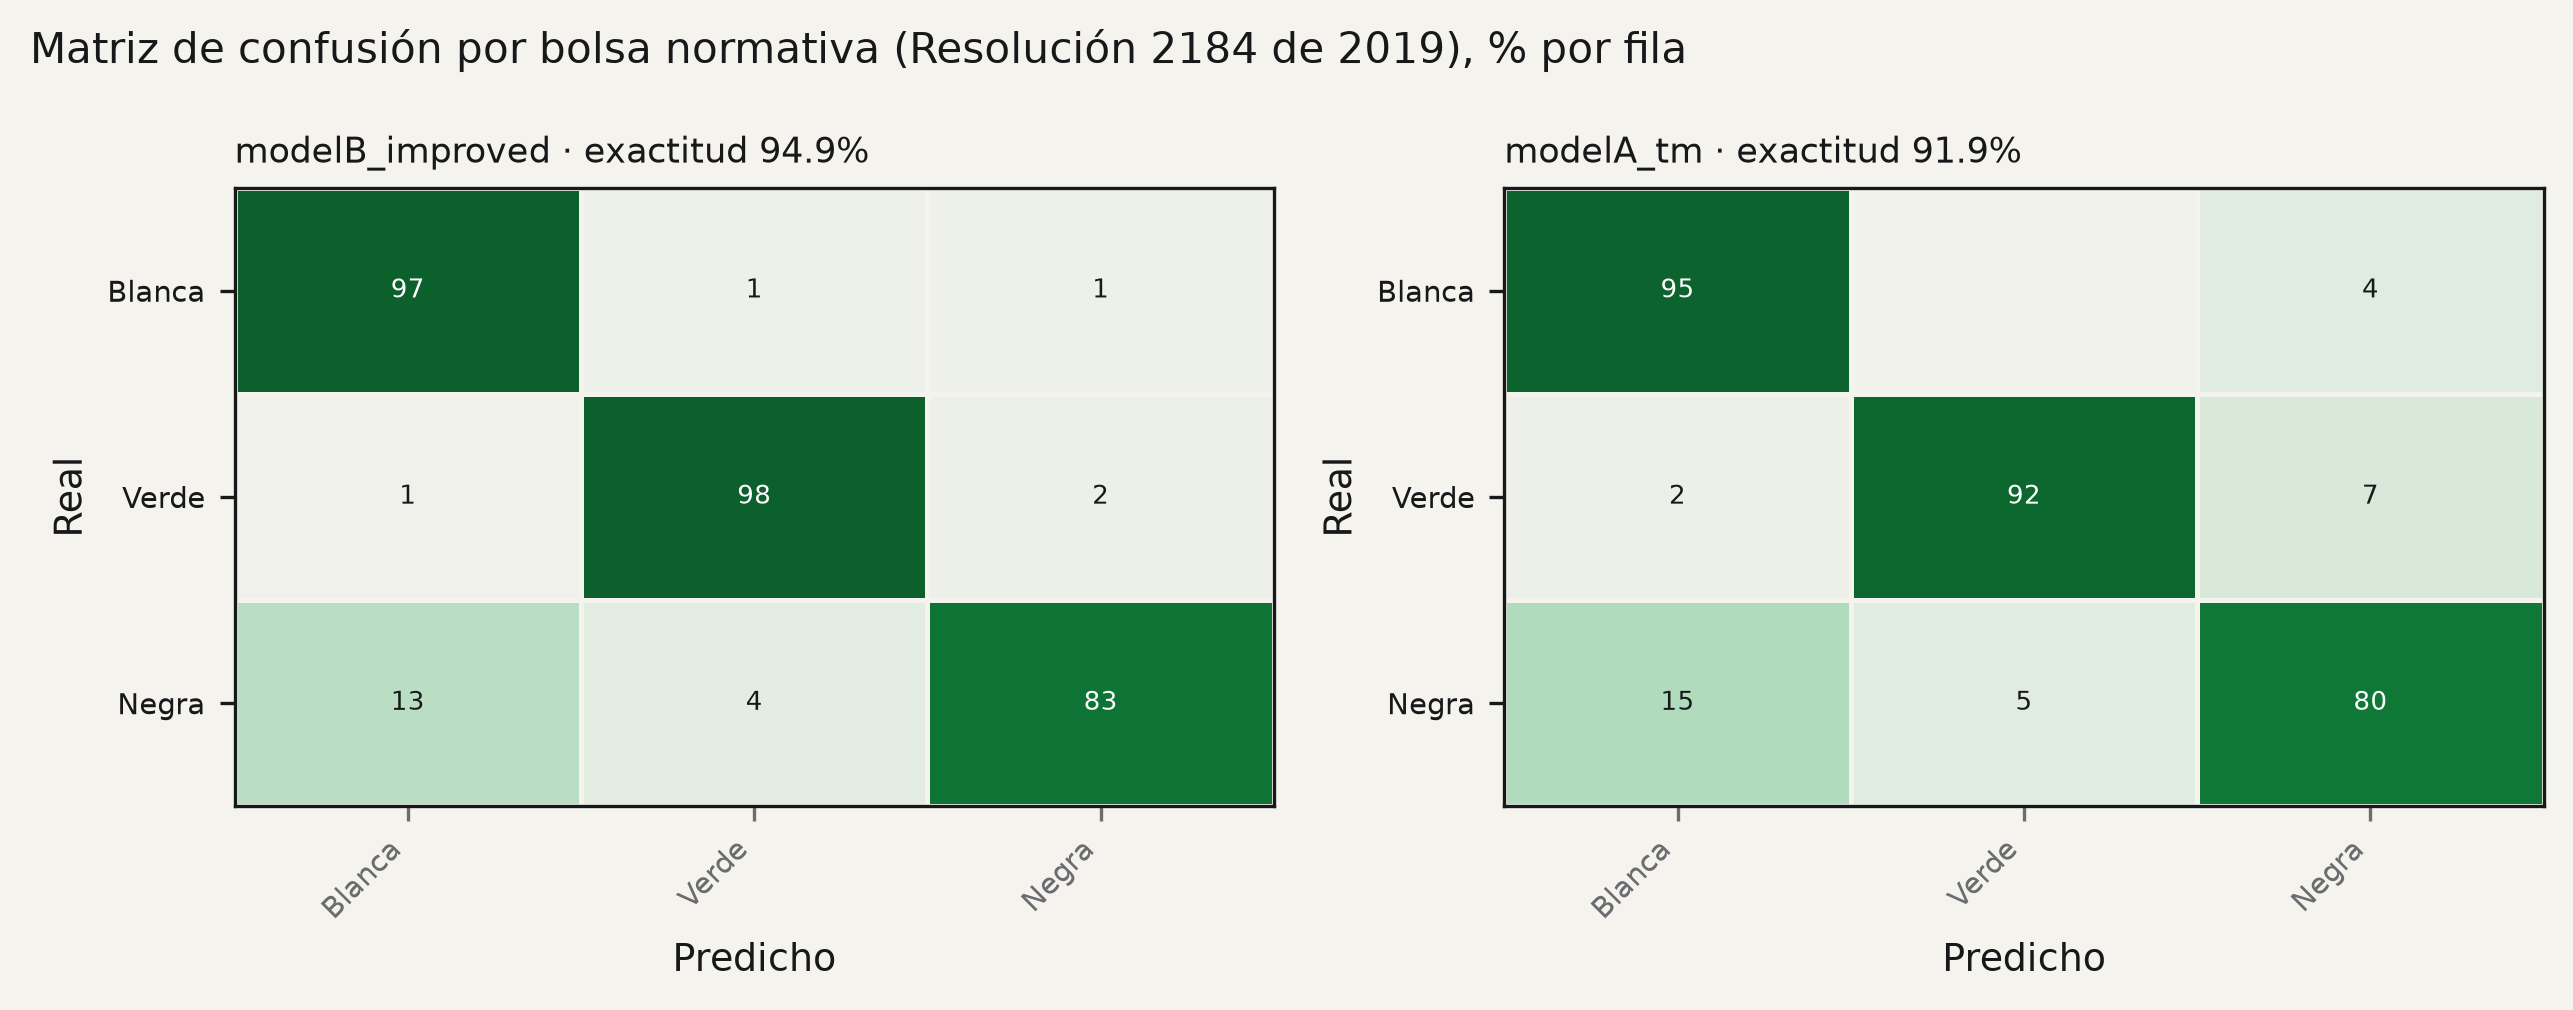
\includegraphics[width=0.88\textwidth]{matriz_bolsas.png}
\caption{Matrices de confusi\'on de bolsas: Modelo A (izquierda) y Modelo B
(derecha).}
\label{fig:matriz_bolsas}
\end{figure*}

\subsection{ROC y separaci\'on por clase}

La Fig.~\ref{fig:roc} muestra las curvas ROC uno-contra-el-resto del Modelo B. El
AUC macro es 0,987; la clase m\'as baja es Pl\'astico (0,970) y la m\'as alta,
Vegetaci\'on (1,000). Un AUC alto con recall bajo en Pl\'astico no es
contradictorio: el modelo ordena bien las probabilidades, pero el umbral de
decisi\'on de 0,5 impl\'icito en el argmax deja fuera casos que est\'an cerca del
l\'imite. La Tabla~\ref{tab:clases} permite comparar el F1 de los dos modelos
clase por clase.

\begin{figure}[!tb]
\centering
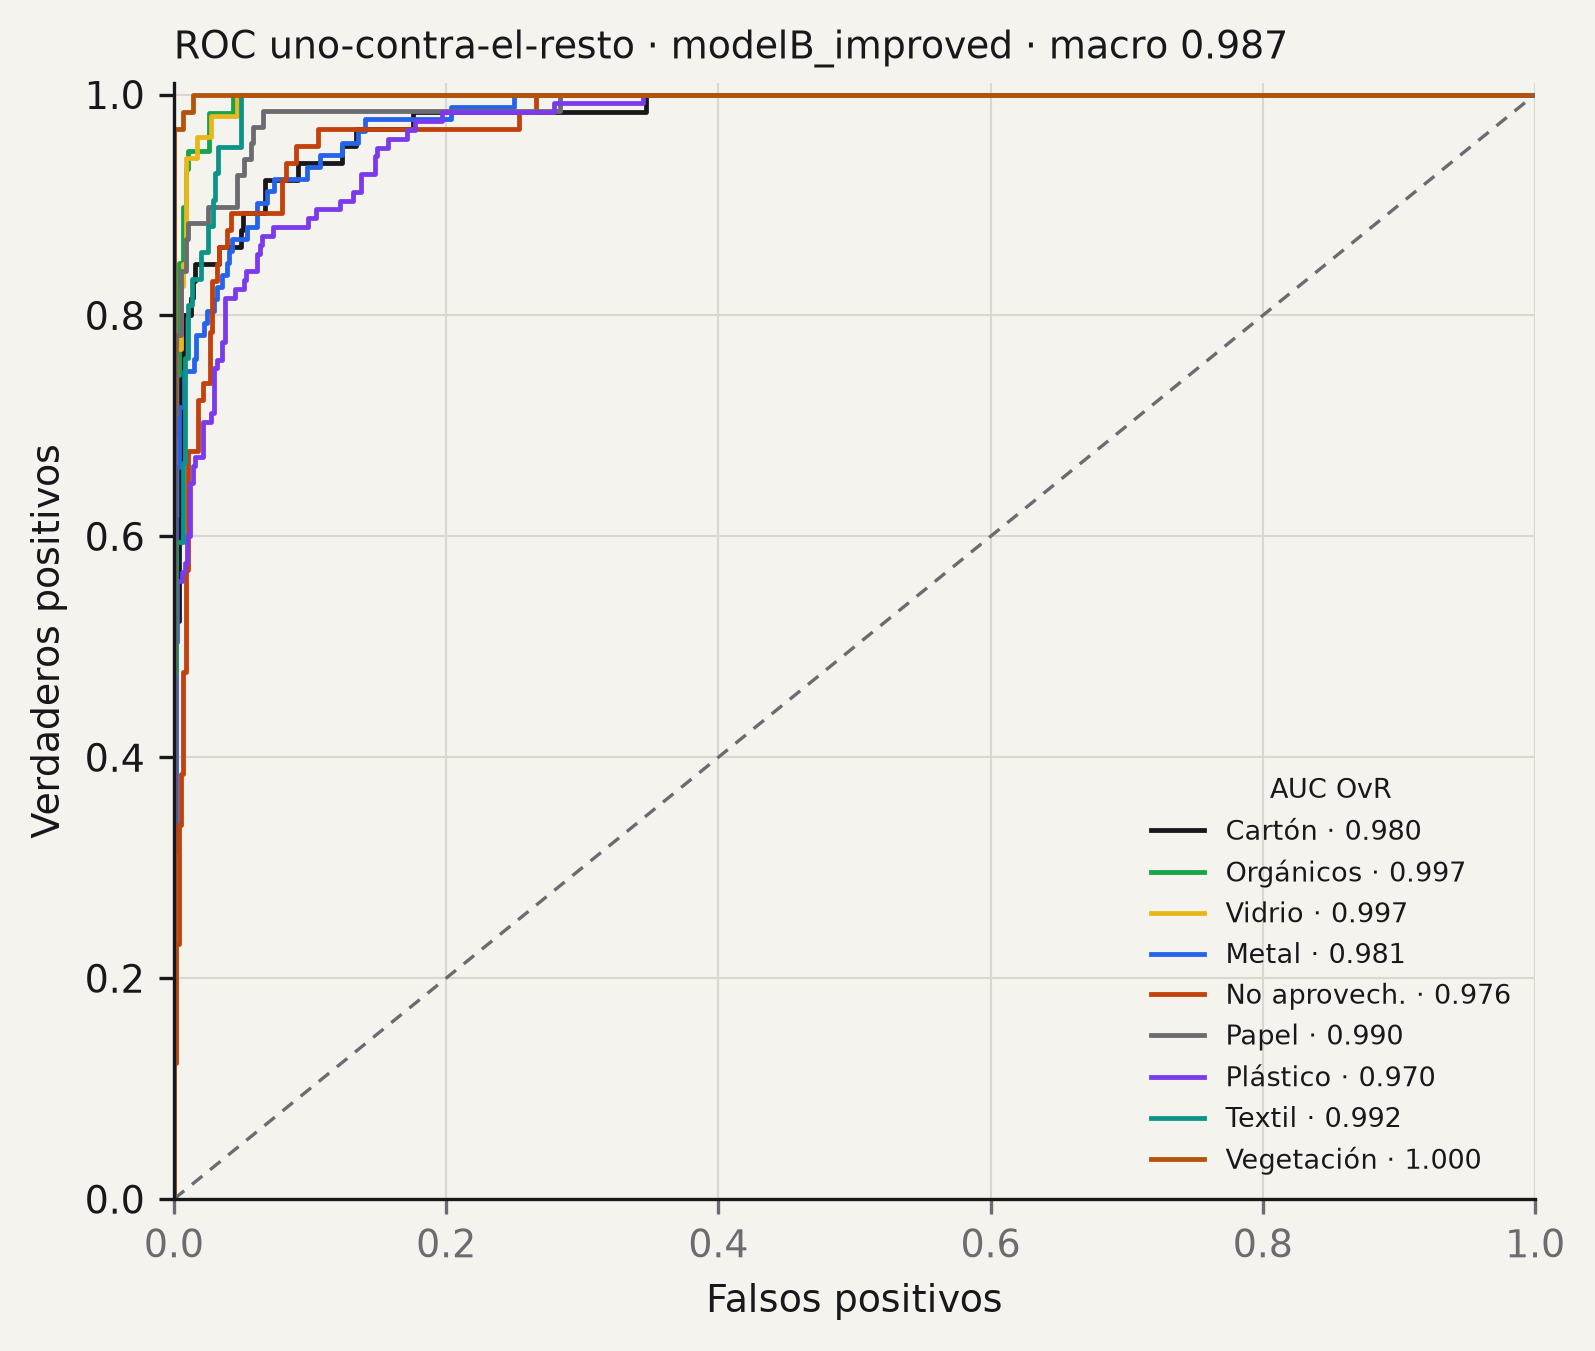
\includegraphics[width=0.86\columnwidth]{roc_b.png}
\caption{Curvas ROC uno-contra-el-resto del Modelo B en \texttt{test/}.}
\label{fig:roc}
\end{figure}

\subsection{Abstenci\'on}

La Fig.~\ref{fig:cobertura} muestra la curva cobertura--exactitud sobre
\texttt{val/}. El punto elegido, $\tau=0{,}63$, acepta el 77,6\,\% de las
im\'agenes con 90,0\,\% de material y 96,5\,\% de bolsa correctos. Al aplicarlo a
\texttt{test/}, el Modelo B decide en el 80,9\,\% de los casos y, entre esos,
acierta el 91,8\,\% del material y el 98,2\,\% de la bolsa. El Modelo A, con el
mismo umbral, decide en el 92,3\,\% pero solo acierta el 81,5\,\% del material: su
confianza no est\'a calibrada y el umbral no lo protege. La Tabla~\ref{tab:abst}
resume los puntos de operaci\'on.

\begin{table}[t]
\centering
\caption{Efecto del umbral $\tau=0{,}63$ sobre validaci\'on y prueba.}
\label{tab:abst}
\footnotesize
\setlength{\tabcolsep}{4pt}
\begin{tabular}{@{}llrrr@{}}
\toprule
Modelo & Conjunto & Cobertura & Mat. & Bolsa \\
\midrule
B & val (calibraci\'on) & 0,776 & 0,900 & 0,965 \\
B & test & 0,809 & 0,918 & 0,982 \\
A & test & 0,923 & 0,815 & 0,942 \\
\bottomrule
\end{tabular}
\end{table}

\begin{figure}[!tb]
\centering
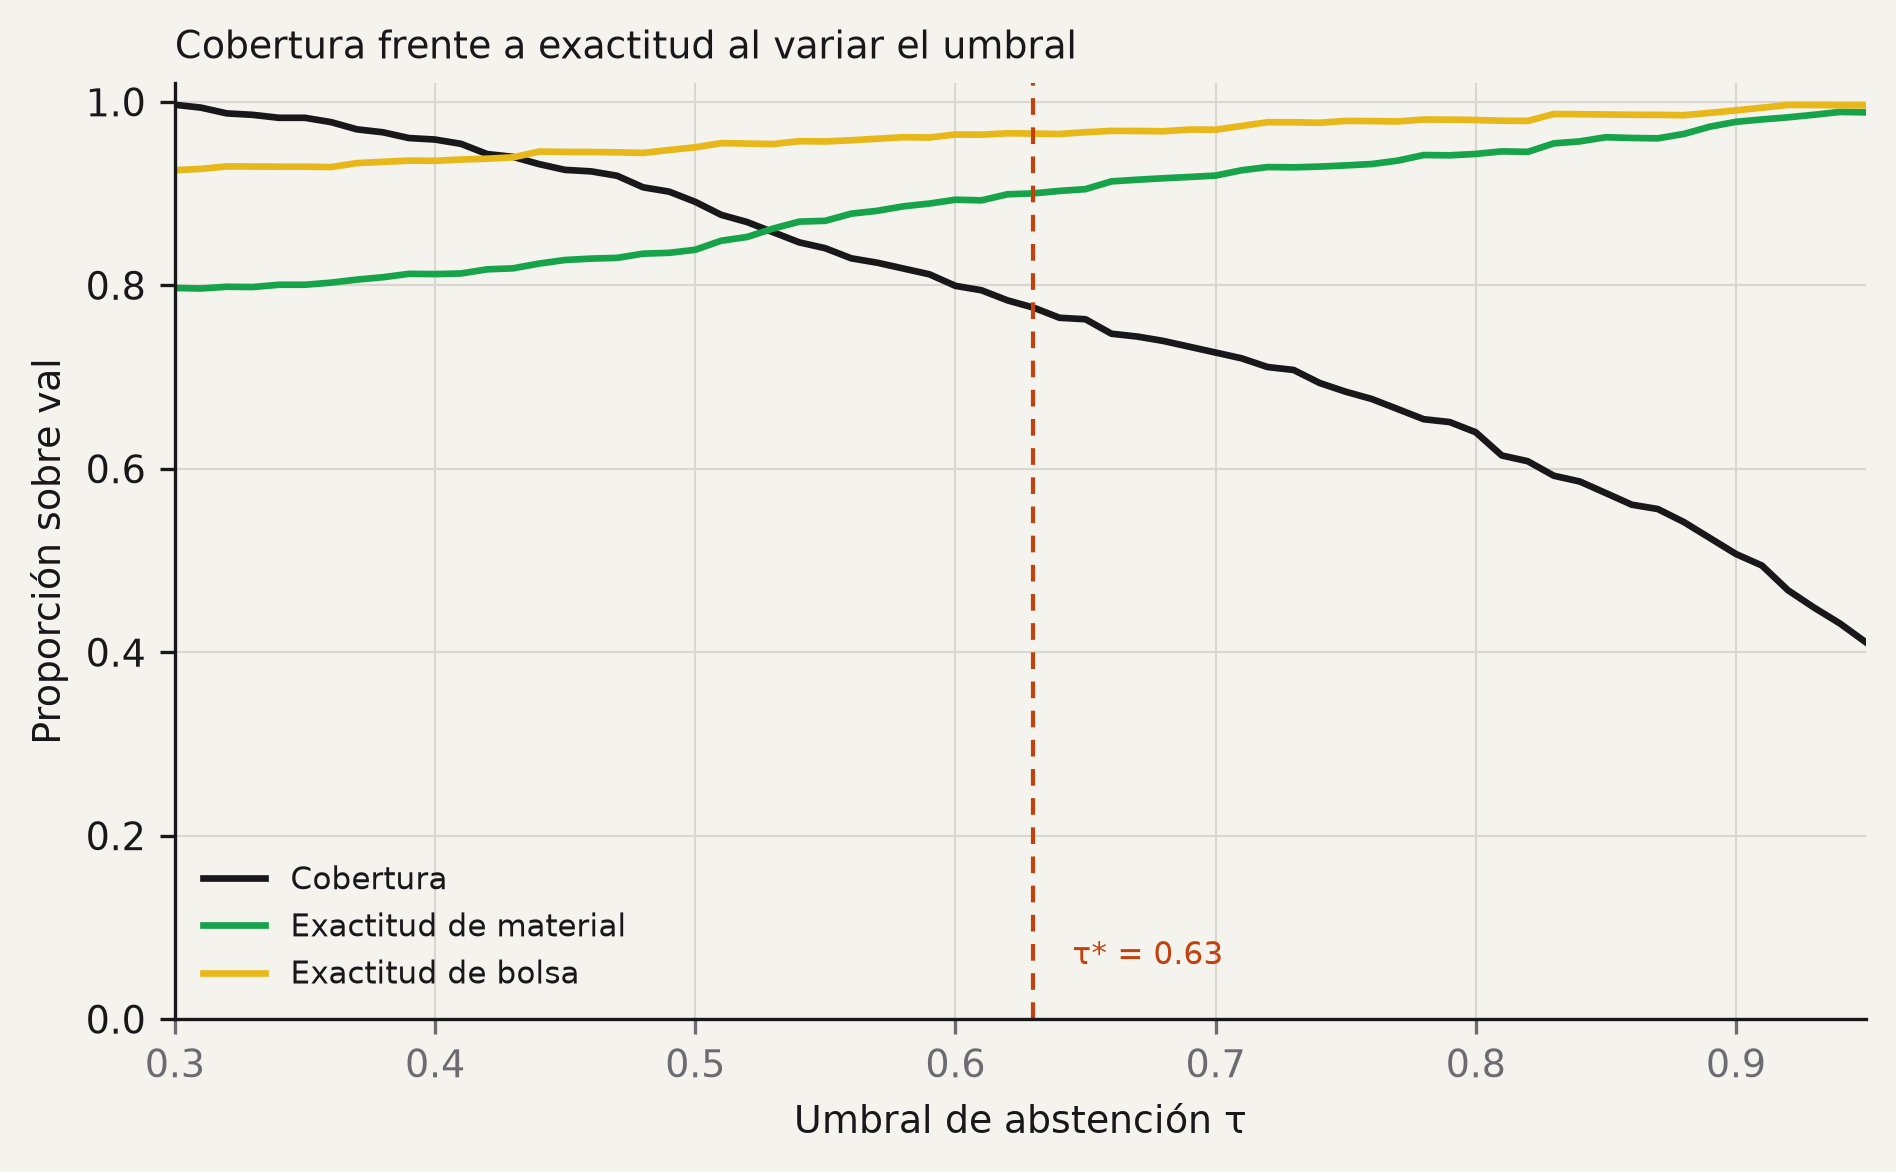
\includegraphics[width=\columnwidth]{cobertura_umbral.png}
\caption{Cobertura frente a exactitud de material y de bolsa al mover $\tau$
sobre \texttt{val/}. El punto marca $\tau=0{,}63$.}
\label{fig:cobertura}
\end{figure}

\subsection{Cambio de dominio con TrashNet}

La Tabla~\ref{tab:trashnet} y la Fig.~\ref{fig:trashnet} reportan la prueba
externa. La exactitud de material del Modelo B cae al 42,4\,\% sobre las cinco
clases compartidas; el A queda en 41,1\,\%. La ca\'ida es esperable: TrashNet
tiene fondo blanco, objetos centrados y una distribuci\'on distinta. A nivel de
bolsa, el B acierta el 92,9\,\% y el A el 87,2\,\%, pero esa cifra est\'a inflada
porque 2.390 de las 2.527 im\'agenes van a la blanca; la F1 macro de bolsa del B
es solo 0,349 y su recall en la negra, 0,058. La conclusi\'on honesta es que el
modelo no generaliza a un dominio fotogr\'afico distinto sin ajuste, y que la
exactitud de bolsa no debe leerse sin la matriz.

Con abstenci\'on, el B acepta el 57,7\,\% de TrashNet y sube al 49,0\,\% de
material; el A acepta el 87,9\,\% y sube al 42,6\,\%. El umbral filtra algo de
ruido, pero no repara el cambio de dominio.

\begin{table*}[t]
\centering
\caption{Prueba externa con TrashNet (2.527 im\'agenes; material sobre las cinco
clases compartidas, 2.390).}
\label{tab:trashnet}
\footnotesize
\setlength{\tabcolsep}{5pt}
\begin{tabular}{@{}lrrrrrr@{}}
\toprule
Modelo & Mat. acc & F1 mat. & Cob. & Mat.$\mid$aceptada & Bolsa acc & F1 bolsa macro \\
\midrule
A & 0,411 & 0,437 & 0,879 & 0,426 & 0,872 & 0,348 \\
B & \textbf{0,424} & 0,420 & 0,577 & \textbf{0,490} & \textbf{0,929} & 0,349 \\
\bottomrule
\end{tabular}
\end{table*}

\begin{figure*}[t]
\centering
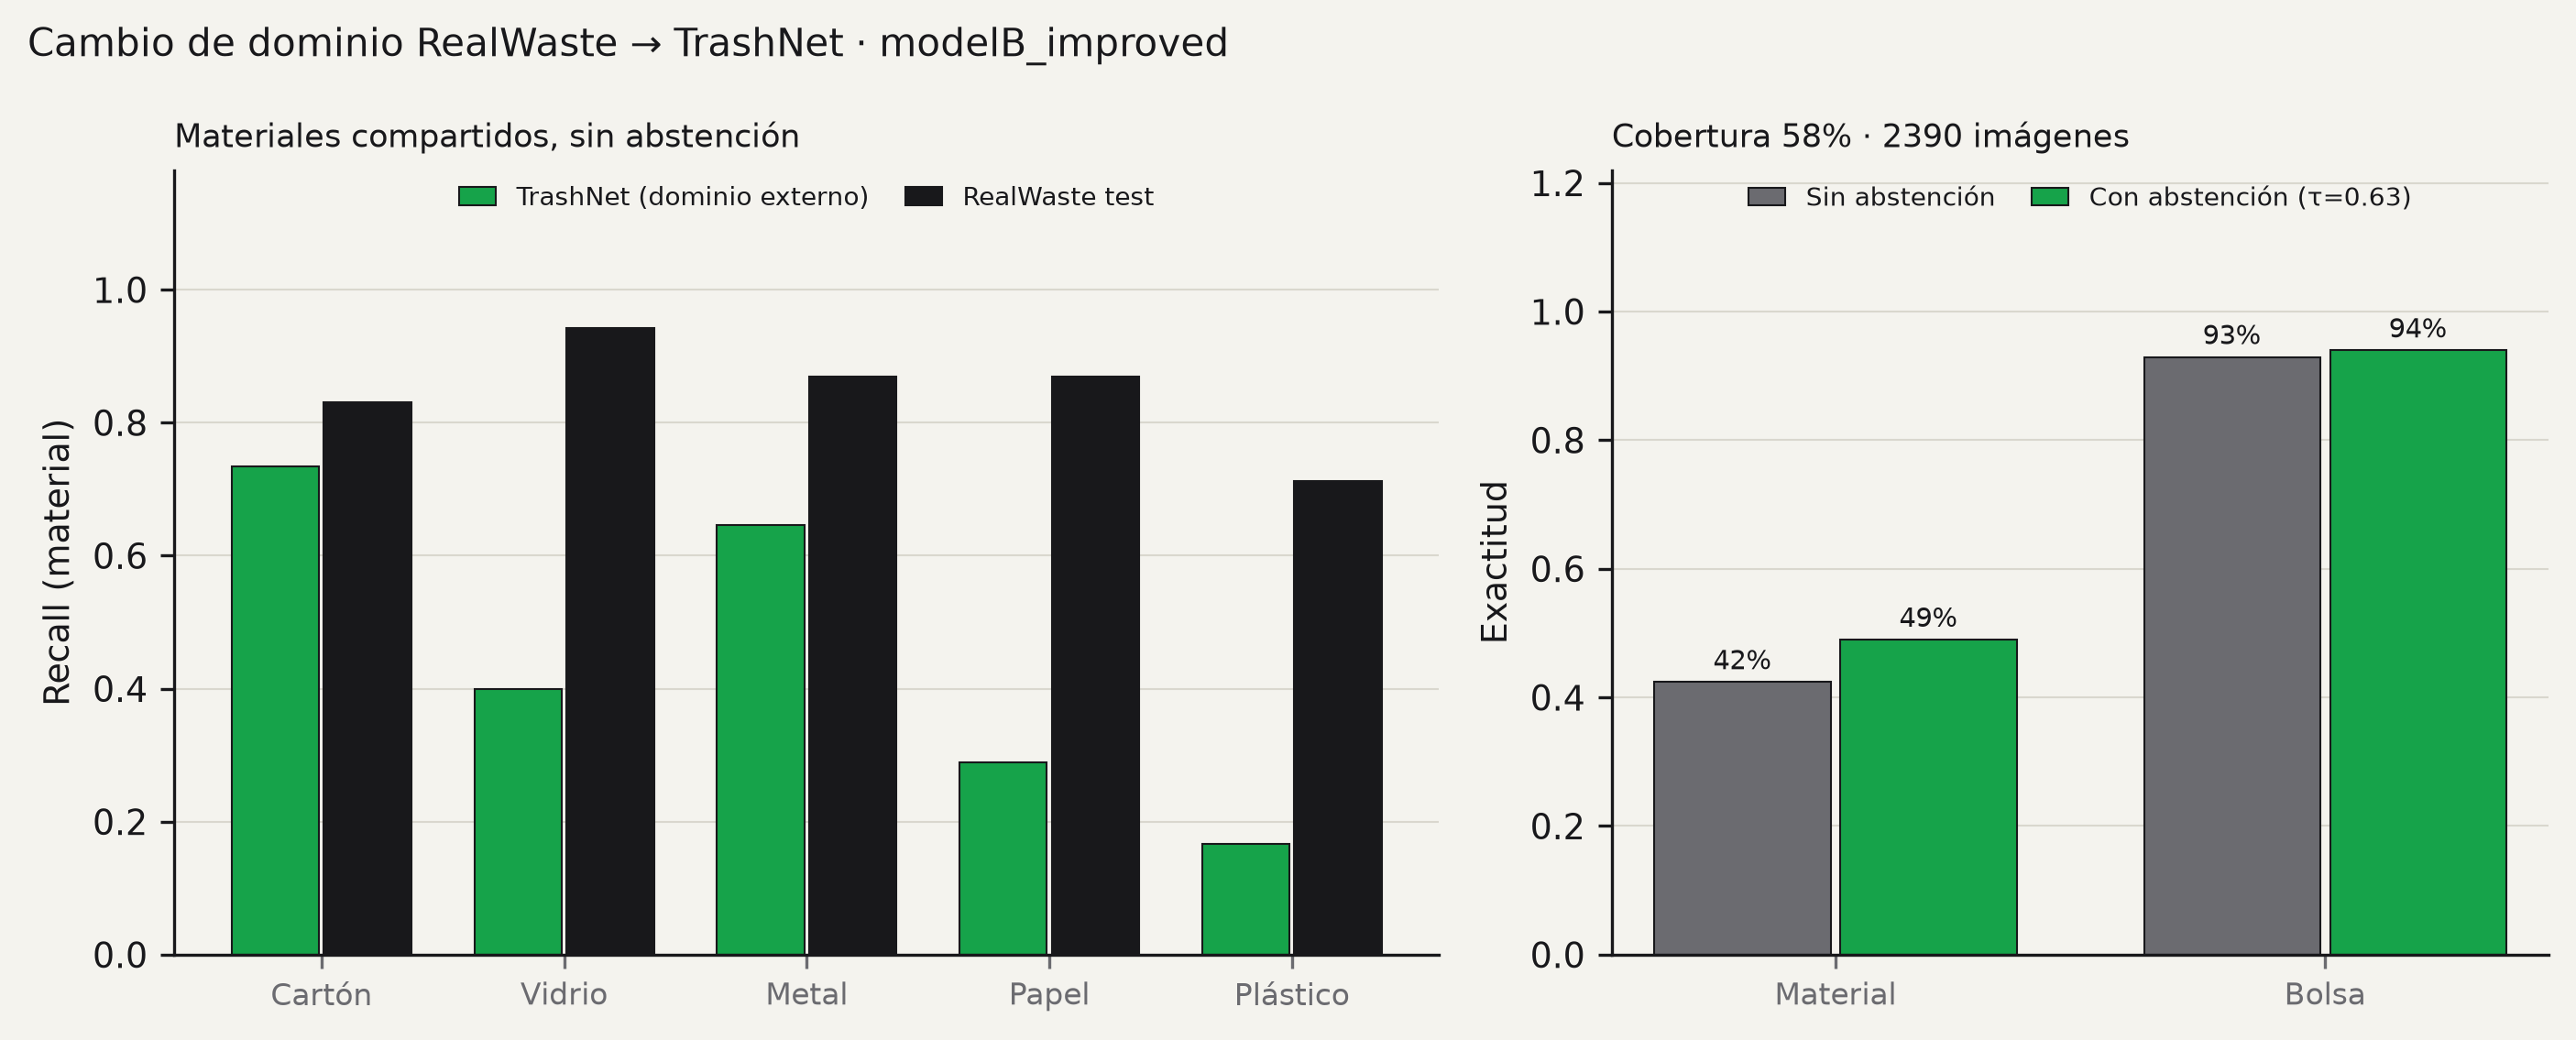
\includegraphics[width=0.9\textwidth]{trashnet_b.png}
\caption{Recall por material en TrashNet frente a \texttt{test/} para el Modelo B,
con y sin abstenci\'on.}
\label{fig:trashnet}
\end{figure*}

\subsection{Latencia y despliegue}

En el VPS, la inferencia de una imagen tarda entre 5 y 12 ms en CPU, incluido el
preprocesado; una pasada completa por las 633 im\'agenes de \texttt{test/} tarda
alrededor de 10 s en el equipo de desarrollo, es decir, unos 16 ms por imagen con
decodificaci\'on y redimensionado. La imagen Docker pesa 471 MB, corre como
usuario sin privilegios y responde \texttt{healthy} en el health check. El
contenedor no publica puertos: solo lo alcanza Traefik por la red \texttt{web}. El
certificado Let's Encrypt se emiti\'o en el cuarto intento del primer despliegue
(unos 24 s) y HTTP redirige a HTTPS con 301. El pipeline completo, desde el push
hasta el health check, tarda alrededor de un minuto.

\subsection{An\'alisis de errores}

Los errores del Modelo B se concentran en tres fronteras. La primera es
Pl\'astico--Metal: envases metalizados, bolsas brillantes y latas arrugadas
comparten reflejos y formas. La segunda es No aprovechable--Textil: la clase
negra mezcla telas, cuerdas y objetos sucios que no comparten una textura com\'un.
La tercera es Cart\'on--Papel: cajas h\'umedas o con impresi\'on se parecen al
papel grueso. A nivel de bolsa, la mayor\'ia de esos errores se perdona porque los
dos materiales van a la blanca; el que m\'as duele es el paso de negra a blanca,
que contamina el flujo aprovechable. Ese es el error que la abstenci\'on deber\'ia
capturar y el que la interfaz se\~nala cuando la confianza no alcanza.

\subsection{El costo asim\'etrico de los errores}
\label{sec:costo}

Las matrices de bolsas de la Fig.~\ref{fig:matriz_bolsas} se pueden leer en
t\'erminos de costo y no solo de acierto. Un residuo que cae en la bolsa blanca
cuando deb\'ia ir a la negra contamina el flujo aprovechable y puede invalidar una
bolsa entera; uno que cae en la negra cuando era aprovechable pierde valor, pero
no contamina. La Tabla~\ref{tab:costo} cuenta los dos tipos de error sin
abstenci\'on, con el mismo criterio para los dos modelos.

\begin{table}[t]
\centering
\caption{Errores de bolsa por tipo, sin abstenci\'on. Porcentaje sobre el
soporte real de cada bolsa (107 negra, 403 blanca, 123 verde).}
\label{tab:costo}
\footnotesize
\setlength{\tabcolsep}{4pt}
\begin{tabular}{@{}lrrr@{}}
\toprule
Modelo & Negra$\rightarrow$Aprov. & Blanca$\rightarrow$Negra & Verde$\rightarrow$Negra \\
\midrule
A & 21 (19,6\,\%) & 18 (4,5\,\%) & 8 (6,5\,\%) \\
B & 18 (16,8\,\%) & 6 (1,5\,\%) & 2 (1,6\,\%) \\
\bottomrule
\end{tabular}
\end{table}

El Modelo B comete menos errores en las tres direcciones, pero la diferencia no
es uniforme. En la frontera peligrosa, el paso de negra a blanca o verde, los dos
modelos est\'an cerca (18 y 21 casos de 107, alrededor de uno de cada cinco): la
bolsa negra sigue siendo el punto d\'ebil del sistema y ninguno de los dos puede
declararse confiable en ella. Donde el B se separa es en el error opuesto: manda
a la negra 6 residuos aprovechables frente a 18 del A, y 2 org\'anicos frente a 8.
Para el usuario, esa diferencia es la que decide si el sistema ahorra material o
solo lo entierra. La asimetr\'ia tambi\'en justifica el umbral: la abstenci\'on no
repara la frontera negra, pero evita decidir cuando la evidencia es d\'ebil, que
es lo \'unico que un clasificador puede prometer con honestidad.

% ============================================================================
\section{Discusi\'on}
\label{sec:discusion}

\subsection{Por qu\'e gana el Modelo B}

La diferencia no proviene de la arquitectura solamente. El Modelo B ve 2.951
im\'agenes frente a 1.620 del A, usa aumento de datos, compensa el desbalance con
pesos por clase y ajusta dos bloques de caracter\'isticas con un planificador
coseno. El Modelo A, en cambio, usa la configuraci\'on predeterminada de una
herramienta sin c\'odigo y no puede compensar el desbalance. La comparaci\'on es
justa para el objetivo del trabajo: mide lo que un equipo obtiene con cada
camino, no dos arquitecturas aisladas. Aun as\'i, el A no es un modelo trivial:
alcanza 0,919 de exactitud de bolsa y 0,971 de AUC, y su principal problema es la
calibraci\'on, no la separaci\'on.

\subsection{La capa normativa y la elecci\'on de la m\'etrica}

El resultado m\'as importante del trabajo no es una exactitud sino una separaci\'on
de responsabilidades. El modelo aprende apariencia; la norma decide el destino. Esa
divisi\'on permite reportar dos niveles y entender por qu\'e la exactitud de bolsa
es alta incluso cuando el material falla. Tambi\'en explica por qu\'e el umbral se
calibra sobre material: si se calibrara sobre bolsa, el sistema aceptar\'ia casi
todo y la abstenci\'on ser\'ia un adorno. La curva de la Fig.~\ref{fig:cobertura}
hace visible ese compromiso y permite elegir otro punto si el contexto lo exige.

\subsection{El cambio de dominio}

TrashNet muestra el l\'imite del prototipo. Un modelo entrenado en un relleno
sanitario no se transfiere sin m\'as a fotos de estudio con fondo blanco. La
ca\'ida al 42,4\,\% de material no invalida el sistema para su dominio, pero s\'i
obliga a declarar que la aplicaci\'on est\'a pensada para fotos de objetos reales,
idealmente sobre una superficie neutra y con buena luz. La prueba tambi\'en
recuerda que la exactitud de bolsa puede ser enga\~nosa: con el 92,9\,\% de
TrashNet, el recall de la bolsa negra es 0,058. Reportar solo la exactitud global
habr\'ia ocultado esa falla.

\subsection{Limitaciones}

\begin{itemize}
\item Una foto por objeto: el sistema no detecta ni segmenta varios residuos en
una escena; el usuario debe encuadrar uno.
\item Dominio acotado: el entrenamiento viene de un relleno sanitario; el uso
dom\'estico tiene fondos, luces y escalas distintas.
\item Clases ambiguas: Pl\'astico, Metal y No aprovechable comparten apariencias
que el corpus no separa del todo.
\item Sin estudio de usuarios: no se midi\'o si la explicaci\'on y la abstenci\'on
mejoran la decisi\'on de una persona.
\item Interfaz solo en espa\~nol y dependiente de HTTPS para la c\'amara.
\item El umbral es global; una calibraci\'on por clase o por bolsa podr\'ia
reducir el costo de los errores m\'as graves.
\end{itemize}

\subsection{Trabajo futuro}

Tres l\'ineas son inmediatas. La primera es la detecci\'on y segmentaci\'on de
m\'ultiples objetos para pasar de una foto por residuo a una escena completa. La
segunda es la calibraci\'on por clase y el uso de predicci\'on conforme, que
ofrece garant\'ias de cobertura sin depender de una softmax sobreconfiada. La
tercera es llevar el modelo al dispositivo con ONNX Runtime Web o una variante
cuantizada, para que la foto no salga del tel\'efono. Tambi\'en queda pendiente un
estudio con usuarios y la extensi\'on a residuos peligrosos y de aparatos
el\'ectricos, que hoy no tienen cabida en las tres bolsas.

\subsection{Reproducibilidad y deuda t\'ecnica}

El proyecto se vuelve a ejecutar de punta a punta con siete scripts y un
manifiesto: la partici\'on es determinista con semilla fija, est\'a cubierta por
pruebas y las cifras del informe se regeneran con \texttt{s06\_evaluar.py}. Esa
cadena es m\'as valiosa que cualquier resultado puntual, porque convierte cada
afirmaci\'on en algo que otro equipo puede repetir.

La reproducibilidad, sin embargo, tiene dos huecos. El primero es el entorno de
entrenamiento: las versiones de PyTorch, torchvision y tf2onnx quedan fijadas en
la imagen de producci\'on, pero no existe un archivo de bloqueo para el entorno de
desarrollo, y los pesos de ImageNet dependen de torchvision. El segundo es el
registro de modelos: los ONNX se guardan en \texttt{models/} sin un hash ni una
ficha que los ligue a la partici\'on que los produjo. Ninguno de los dos afecta
las cifras de este informe, pero ambos son la primera deuda que habr\'ia que
pagar antes de operar el sistema fuera del aula.

En producci\'on tampoco hay monitoreo m\'as all\'a del \texttt{health check}:
\'este confirma que el proceso responde y que el ONNX carga, no que las
predicciones sigan siendo buenas. Un despliegue real necesitar\'ia registrar la
confianza de las respuestas y revisar muestras peri\'odicamente para detectar el
deterioro por cambio de dominio que TrashNet ya anticipa.

% ============================================================================
\section{Conclusiones}
\label{sec:conclusiones}

El trabajo construy\'o un clasificador de residuos que responde con la bolsa
normativa de la Resoluci\'on 2184 de 2019 y que se abstiene cuando la evidencia no
alcanza. La separaci\'on entre la predicci\'on del material y la regla normativa
result\'o clave: permiti\'o comparar los modelos con m\'etricas de la literatura,
reportar la decisi\'on real y mantener la norma fuera del entrenamiento.

Sobre las 633 im\'agenes de prueba, el Modelo B obtuvo 83,6\,\% de exactitud de
material, 94,9\,\% de bolsa, 0,841 de F1 macro y 0,987 de AUC; el Modelo A,
78,2\,\%, 91,9\,\%, 0,777 y 0,971. El umbral calibrado en validaci\'on,
$\tau=0{,}63$, dej\'o al B decidiendo en el 80,9\,\% de los casos con 91,8\,\% de
material y 98,2\,\% de bolsa correctos. El A, con el mismo umbral, decidi\'o en
el 92,3\,\% pero solo acert\'o el 81,5\,\% del material: la calibraci\'on, y no
solo la exactitud, separa a los dos modelos.

La prueba externa con TrashNet baj\'o la exactitud de material al 42,4\,\%, lo
que delimita el alcance: el prototipo funciona en su dominio y no reemplaza un
sistema de producci\'on sin ajuste. El despliegue en un VPS real, con TLS,
contenedor sin privilegios, CI/CD y un umbral visible en la interfaz, demuestra
que el flujo completo es reproducible y que las cifras del informe se pueden
volver a comprobar con los scripts del repositorio.

Como trabajo inmediato queda la detecci\'on de m\'ultiples objetos, la
calibraci\'on por clase y una evaluaci\'on con usuarios. El prototipo no sustituye
la norma ni la decisi\'on de la autoridad ambiental, pero s\'i muestra que un
sistema puede decir ``no s\'e'' cuando no sabe, que es la conducta m\'as honesta
frente a un residuo que puede contaminar una bolsa entera.

% ============================================================================
\begin{acknowledgments}
Los autores agradecen a la Maestr\'ia en Inteligencia Artificial de la Universidad
de La Salle por el acompa\~namiento durante el desarrollo del proyecto.
\end{acknowledgments}

\clearpage
\bibliographystyle{IEEEtran}
\bibliography{refs}

% ============================================================================
\appendix

\section{Reproducibilidad}
\label{app:repro}

El repositorio se ejecuta en el siguiente orden. Los dos primeros pasos solo
necesitan las dependencias de desarrollo; el entrenamiento del Modelo A y la
conversi\'on a ONNX requieren TensorFlow y \texttt{tf2onnx}, que no se instalan en
producci\'on.

\begin{verbatim}
python src/s01_datos.py
python src/s02_eda.py
python src/s02_tm.py
python src/s03_convertir_onnx.py
python src/s04_modelo_b.py
python src/s05_calibrar_umbral.py
python src/s06_evaluar.py
\end{verbatim}

Las pruebas se ejecutan con \texttt{pytest} y cubren datos, dominio, imagen,
inferencia y contrato. La aplicaci\'on local se levanta con
\texttt{uvicorn app:app --app-dir api --port 8000} despu\'es de compilar el
frontend con \texttt{trunk build --release} en \texttt{web/}. La imagen se
construye con \texttt{docker build -t residuos-2184 .} y se sirve en el puerto
8000.

\section{Respuesta del contrato}
\label{app:json}

La respuesta de \texttt{/api/predict} tiene la forma siguiente. Los colores se
incluyen para que la interfaz no tenga que duplicar la tabla normativa.

{\footnotesize
\begin{verbatim}
{
  "material": "Plastico", "bolsa": "blanca",
  "bolsa_nombre": "Blanca", "confianza": 0.87,
  "abstenido": false,
  "top3": [{"material": "Plastico", "p": 0.87}],
  "bolsas_prob": {"blanca": 0.91, "verde": 0.02,
                  "negra": 0.07},
  "latencia_ms": 8.4
}
\end{verbatim}

\end{document}
